%%%%%%%%%%%%%%%%%%%%%%%%%%%%%%%%%%%%%%%%%%%%%%%%%%%
%% LaTeX book template                           %%
%% Author:  Amber Jain (http://amberj.devio.us/) %%
%% License: ISC license                          %%
%%%%%%%%%%%%%%%%%%%%%%%%%%%%%%%%%%%%%%%%%%%%%%%%%%%

\documentclass[a4paper,11pt]{book}
\usepackage[T1]{fontenc}
\usepackage[utf8]{inputenc}
\usepackage{lmodern}
%%%%%%%%%%%%%%%%%%%%%%%%%%%%%%%%%%%%%%%%%%%%%%%%%%%%%%%%%
% Source: http://en.wikibooks.org/wiki/LaTeX/Hyperlinks %
%%%%%%%%%%%%%%%%%%%%%%%%%%%%%%%%%%%%%%%%%%%%%%%%%%%%%%%%%
\usepackage{/Users/HechenHu/Development/NoteTaking/Mathematics-Notes/Customized}
\graphicspath{ {/Users/HechenHu/Development/NoteTaking/Mathematics-Notes/Point-Set\_Topology} }
%%%%%%%%%%%%%%%%%%%%%%%%%%%%%%%%%%%%%%%%%%%%%%%%
% Chapter quote at the start of chapter        %
% Source: http://tex.stackexchange.com/a/53380 %
%%%%%%%%%%%%%%%%%%%%%%%%%%%%%%%%%%%%%%%%%%%%%%%%

\makeatletter

\renewcommand{\@chapapp}{}% Not necessary...

\newenvironment{chapquote}[2][2em]
{\setlength{\@tempdima}{#1}%
	\def\chapquote@author{#2}%
	\parshape 1 \@tempdima \dimexpr\textwidth-2\@tempdima\relax%
	\itshape}
{\par\normalfont\hfill--\ \chapquote@author\hspace*{\@tempdima}\par\bigskip}
\makeatother

%%%%%%%%%%%%%%%%%%%%%%%%%%%%%%%%%%%%%%%%%%%%%%%%%%%
% First page of book which contains 'stuff' like: %
%  - Book title, subtitle                         %
%  - Book author name                             %
%%%%%%%%%%%%%%%%%%%%%%%%%%%%%%%%%%%%%%%%%%%%%%%%%%%

% Book's title and subtitle
\title{\Huge \textbf{Point-Set Topology}}
% Author
\author{\textsc{Hechen Hu}}

\begin{document}
	\frontmatter
	\maketitle
	%%%%%%%%%%%%%%%%%%%%%%%%%%%%%%%%%%%%%%%%%%%%%%%%%%%%%%%%%%%%%%%%%%%%%%%%
	% Auto-generated table of contents, list of figures and list of tables %
	%%%%%%%%%%%%%%%%%%%%%%%%%%%%%%%%%%%%%%%%%%%%%%%%%%%%%%%%%%%%%%%%%%%%%%%%
	
	\tableofcontents
	\mainmatter
	
	\chapter{Basic Set Theory}
	\section{Classification of Relations}
	\begin{Definition}
		An \textit{equivalence relation} is a relation that satisfy the following properties: \\
		\newline
		$ aRa $ (Reflexivity);\\
		$ aRb \Rightarrow bRa $ (Symmetry); \\
		$ (aRb)\land (bRc) \Rightarrow aRc $ (Transitivity).\\
		\newline
		An equivalence relation is denoted by the special symbol $ \sim $. $ a\sim b $ means $ a $ is \textit{equivalent} to $ b $.	
	\end{Definition}
	\begin{Definition}
		Let $ R(\sim) $ be an equivalence relation on $ A $. If $ a \in A $, the \textit{equivalence class} of $ a $ (denoted $ \bar{a} $) is the class of all those elements of $ A $ that are equivalent to $ a $. The class of all equivalence classes in $ A $ is denoted $ A/R $ and called the \textit{quotient class} of $ A $ by $ R $.
	\end{Definition}
	\begin{Theorem}
		Two equivalence classes are either disjoint or equal.
	\end{Theorem}
	
	\begin{Definition}
		A \textit{partial ordering} on a set $ X^2 $ is a relation $ R $ that have the following properties: \\
		\newline
		$ aRa $ (Reflexivity);\\
		$ (aRb)\land (bRc) \Rightarrow aRc $ (Transitivity).\\
		$ (aRb) \land (bRa )\Rightarrow (a=b) $ (Anti-symmetry);	
	\end{Definition}
	
	We often write $ a\preceq b $ and say that $ b $ \textit{follows} $ a $.
	If the condition
	\begin{equation}
	\forall a \forall b((aRb)\lor(bRa) \nonumber
	\end{equation}
	holds in addition to transitivity and anti-symmetry defining a partial ordering relation(this means any two elements of $ X $ is comparable), the relation $ R $ is called an \textit{ordering}, and the set $ X $ is said to be \textit{linearly ordered}.
	\begin{Definition}
		A relation $ \prec $ is called a \textit{strict partial order} if it's nonreflexive and transitive.
	\end{Definition}
	\begin{Theorem}[The Maximum Principle]
		Let $ A $ be a set and $ \prec $ be a strict partial order on $ A $. Then there exists a maximal simply ordered(linearly ordered) subset of $ A $.
	\end{Theorem}
	\begin{Lemma}[Zorn's Lemma]
		Let $ A $ be a set that is strictly partially ordered. If every simply ordered subset of $ A $ has an upper bound in $ A $, then $ A $ has a maximal element.
	\end{Lemma}
	\begin{Definition}
		If $ X $ is a set and $ < $ is an order relation on $ X $, and if $ a<b $, the notation $ (a,b) $ to denote the set
		\begin{equation}
		\{x|a<x<b \} \nonumber
		\end{equation}
		it is called an \textit{open interval} in $ X $. If this set is empty, $ a $ is called the \textit{immediate predecessor} of $ b $, and $ b $ is called the \textit{immediate successor} of $ a $.
	\end{Definition}
	\begin{Definition}
		Suppose that $ A $ and $ B $ are two sets with order relations $ <_A $ and $ <_B $ respectively. We say that $ A $ and $ B $ have the same \textit{order type} if there is a bijective correspondence between them that preserves order, that is, if $ f:A \to B $ is a bijection
		\begin{equation}
		a_1 <_A a_2 \Rightarrow f(a_1)<_B f(a_2) \nonumber
		\end{equation}
	\end{Definition}
	\begin{Example}
		The interval $ (1,1) $ of real numbers has the same order type as $ \Real $, for the function $ f:(-1,1)\to \Real $ given by
		\begin{equation}
		f(x)=\frac{x}{1-x^2} \nonumber
		\end{equation}
		is an order-preserving bijection.
	\end{Example}
	\begin{Definition}
		Suppose $ A $ and $ B $ are two sets with order relations $ <_A $ and $ <_B $ respectively. Define an order relation $ < $ on $ A \times B $ by defining
		\begin{equation}
		a_1 \times b_1 < a_2 \times b_2
		\end{equation}
		if $ a_1 <_A a_2 $, or if $ a_1 = a_2 $ and $ b_1 <_B b_2 $. It is called the \textit{dictionary order relation} on $ A \times B $.
	\end{Definition}
	
	\subsubsection{Functions and Their Graphs}
	\begin{Definition}
		A relation $ R $ is said to be functional if
		\begin{equation}
		(xRy_1)\land(xRy_2)\Rightarrow (y_1=y_2) \nonumber
		\end{equation}
		and it is called a \textit{function}.\\
		$ R\subset X \times Y $ is a \textit{mapping from $ X $ into $ Y $}, or a \textit{function from $ X $ into $ Y $}.\\
	\end{Definition}
	\section{Sets and Operations on Them}
	
	\subsection{Naive Set Theory}
	1$^0$.\quad A set may consist of any distinguishable objects($x\in A\Rightarrow\exists!x\in A$) \\
	2$^0$.\quad A set is unambiguously determined by the collection of objects that comprise it. \\
	3$^0$.\quad Any property defines the set of objects having that property($A = \{x|P(x)\}\Rightarrow P(A)$). \\ \\
	However, this will lead to Russell's Paradox: \\
	Let's have$P(M) \coloneqq M\notin M$ \\
	Consider the class $K = \{M|P(M)\}$. If so $K$ is not a set, since whether $P(K)$ is true or false, contradiction arises.\\
	
	\subsection{ZFC: Zermelo-Fraenkel Axioms and Axiom of Choice}
	1$^0$.\quad \textbf{(Axiom of Extensionality)} Sets $ A $ and $B$ are equal iff they have the same elements. $ (A=B)\Leftrightarrow(\forall x((x\in A)\Leftrightarrow(x \in B))) $\\
	2$^0$. \quad \textbf{(Axiom of Seperation)} To any set $A$ and any property P there corresponds a set $B$ whose elements are those elements of $A$, and only those, having property P(if $A$ is a set, then $B=\{x\in A|P(x)\}$ is also a set). \\
	3$^0$. \quad \textbf{(Union Axiom)} For any set $ \mathscr{M} $ whose elements are sets there exists a set $\bigcup M$, called the union of $ M $ and consisting of those elements and only those that belong to some element of $ \mathscr{M} $ $ (x\in \bigcup \mathscr{M} \Leftrightarrow \exists X((X\in \mathscr{M})\land (x\in X))) $ \\
	Similarly, the intersection of the set $ \mathscr{M} $ is defined as:
	\begin{equation}
	\bigcap \mathscr{M}  \coloneqq \{x\in \bigcup \mathscr{M} | \forall X((X\in \mathscr{M})\Rightarrow (x\in X))\} \nonumber
	\end{equation}
	4$^0$ \quad \textbf{(Pairing Axiom)} For any sets $ X $ and $ Y $ there exists a set $ Z $ such that $ X $ and $ Y $ are its only elements. \\
	5$^0$ \quad \textbf{(Power Set Axiom)} For any set $ X $ there exists a set $ P(X)$ having each subset of $ X $ as an element, and having no other elements. \\
	\newline
	\begin{Definition}
		The \textit{successor} $X^+$ of the set $ X $ is $X^+ = X\cup \{X\}$.\\
	\end{Definition} 
	\begin{Definition}
		An \textit{inductive} set is a set that $\varnothing$ is one of its elements and the successor of each of its elements aso belongs to it.
	\end{Definition}
	6$^0$ \quad \textbf{(Axiom of Infinity)} There exist inductive sets (Example: $\mathbb{N}_0$).\\ 
	7$^0$ \quad \textbf{(Axiom of Replacement)} Let $ F(x,y) $ be a statement(a formula) such that for every $ x_0 \in X$ there exists a unique object $ y_0 $ such that $ F(x_0,y_0) $ is true. Then the objects $ y $ for which there exists an element $ x\in X $ such that $ F(x,y) $ is true form a set.\\
	And finally, an axiom that is independent of ZF. \\
	\newline
	8$^0$ \quad \textbf{(Axiom of Choice/Zermelo's Axiom)}  Given a collection of disjoint nonempty sets, there exists another set consisting of exactly one element from each element of the original set.
	\begin{Definition}
		A choice function is a function $ f $, defined on a collection $ X $ of nonempty sets, such that for every set $ A $ in $ X $, $ f(A) $ is an element of $ A $.
	\end{Definition}
\begin{Corollary}
	There exists a choice function for any collection of nonempty sets.
\end{Corollary}

	
	
	\subsection{The \textit{Cardinality} of a Set(\textit{Cardinal Numbers})}
	\begin{Definition}
		The set $ X $ is said to be \textit{equipollent} to the set $ Y $ if there exists a bijective mapping of $ X $ onto $ Y $(then $ X\sim Y $).
	\end{Definition}
	\begin{Definition}
		\textit{Cardinality} is a measure of the number of elements of the set. If $ X \sim Y $, we write $ \card X = \card Y $.
	\end{Definition}
	If $ X $ is equipollent to some subset of $ Y $, we say $ \card X\leqslant \card Y $, thus
	\begin{equation}
	(\card X \leqslant \card Y)\coloneqq \exists Z\subset Y (\card X = \card Z) \nonumber
	\end{equation}
	A set is called \textit{finite} if it is not equipollent to any proper subset of itself; otherwise it is called \textit{infinite}. \\
	It has the  properties below:\\
	\newline
	1$^0  \quad (cardX\leqslant \card Y)\land(\card Y \leqslant \card Z)\Rightarrow(\card X \leqslant \card Z)$.\\
	2$^0 \quad (\card X \leqslant \card Y)\land(\card Y \leqslant \card X)\Rightarrow(\card X = \card Y)$(The Schröder–Bernstein theorem).\\
	3$^0 \quad \forall X\forall Y(\card X \leqslant \card Y)\lor(\card Y \leqslant \card X)$(Cantor's theorem).\\
	\newline
	We say $ \card X < \card Y $ if $ (\card X \leqslant \card Y) \land (\card X \neq \card Y)$.\\
	let $ \varnothing $ be the empty set and $ P(X) $ the set of all subsets(thus, the power set) of the set $ X $. Then:
	\begin{Theorem}
		$ \card X < \card P(X) $
	\end{Theorem}
	\begin{proof}
		The assertion is obvious for the empty set, and we shall assume that $ X\neq \varnothing $.\\
		Since $ P(X) $ contains all the one-element subsets of $ X $, $ \card X \leqslant \card P(X)$.\\
		Suppose, contrary to the assertion, that there exists a bijective mapping $ f : X \to P(X) $. Let set $ A = \{x\in X:x\notin f(x)\}$ consisting of the elements $ x \in X $ that do not belong to the set $ f(x)\in P(X) $ assigned to them by the bijection. Because $ A \in P(X) $, there exists $ a\in X $ such that $ f(a) = A $. For the element $ a $ the relation $ a \in A $ or $ a \notin A $ is impossible by the definition of $ A $(Similar to Russell's Paradox).
	\end{proof}
	
	
	
	\subsection{Operations on Sets}
	\begin{tabular}{| l | l | l |}
		\hline
		Notation &Meaning &Definition \\ \hline
		$A\subset B$ &$A$ is a subset of $B$ &$\forall x ((x\in A) \Rightarrow(x\in B))$ \\ \hline
		$A\subsetneq B$ &$A$ is a proper subset of $B$ &$A \neq B \land A \subset B$ \\ \hline
		$A = B$ &$A$ equals to $B$ &$(A \subset B)\land(B \subset A)$ \\ \hline
		$\varnothing$ &Empty Set & $\{x|x\neq x\}$ \\ \hline
		$A \cup B$ &The union of $ A $ and $ B $ &$ \{x|x\in A \lor x\in B\} $ \\
		$ A \cap B $ &The intersection of $ A $ and $ B $ &$ \{x|x\in A \land x\in B\} $ \\ \hline
		$ A\setminus B $ &The difference between $ A $ and $ B $ &$ \{x|x\in A \land x\notin B\} $ \\ \hline
		$ C_M A $ &The complement of $A$ in M &$ \{x|x\in M \land x\notin A\} where A\subset M $ \\ \hline
		$ A \times B $ &The Cartesian Product of $ A $ and $ B $ &$ \{(x,y)|x\in A \land y\in B\} $ \\ \hline
		$ A^2 $ &$ A \times A $ & \\
		\hline
	\end{tabular}
	\newline \\
	In the ordered pair$ z = (x_1,x_2) $ where$ Z = X_1 \times X_2 ,z\in Z,x_1 \in X_1, x_2 \in X_2$, $ x_1 $ is called the \textit{first projection} of the pair $ z $ and denoted  $\proj_1 z $ while $ x_2 $ is called the \textit{second projection} of the pair $ z $ and denoted  $\proj_2 z $.
	
	
	
	
	
	
	
	\section{Countable and Uncountable Sets}
	
	\begin{Definition}
		A set $ X $ is \textit{countable} if it is equipollent with the set $ \Natural $ of natural numbers, that is, $ \card X = \card \Natural $.
	\end{Definition}
	
	\begin{Proposition}
		An infinite subset of a countable set is countable.
	\end{Proposition}
	\begin{proof}
		Let's consider a countable set $ E $. There is a minimal element of $ E_1\coloneqq E $, which we assign to $ 1 \in \Natural $ and denote $ e_1 \in E $. $ E $ is infinite, so $ E_2 \coloneqq E \setminus e_1 $ is not empty. Following the principle of induction, we can construct a injective mapping from $ \{1,2...\} $ to $ \{e_1,e_2,...\} $. \newpara
		Now we have to prove that this mapping is also surjective. Suppose the contrary, that an element $ e \in E$ does not have a natural number assigned to it. The set $ K=\{n \in E | n \leqslant e\} $ is finite, since it's a subset of $ \Natural $ bounded both from below and above. According to our previous construction, we assign $ 1 $ to $ \min K $, denoted as $ e_1 $, and we can acquire a sequence $ e_1, e_2,...e_{k=\card K} $. But $ e_{k=\card K} $ is $ \max K $, and because $ e\in K \land (\forall n\in K (n\leqslant e))$, $ e = \max K$. Therefore $ e = e_k $, or otherwise it will contradict the uniqueness of maximal element.
	\end{proof}
	
	\begin{Proposition}
		The Union of the sets of a finite or countable system of countable sets is also a countable set.
	\end{Proposition}
	\begin{proof}
		Let $ X_1,X_2...,X_n,... $ is a countable system of sets and each set $ X_m = \{x^1_m,...,x^n_m,...\} $ is itself countable. Since $ \forall m\in \Natural (\card (X=\bigcup_{n \in \Natural}X_n) \geqslant X_m)$, $ X $ is an infinite set. The ordered pair $ (m,n) $ identifies the element $ x^n_m \in X_m $. We can construct a mapping, like $ f : \Natural \times \Natural \to \Natural \coloneqq (m,n) \to \frac{(m+n-2)(m+n-1)}{2}+m $, such that it is bijective. Thus $ X $ is countable. Then because $ \card X \leqslant \card \Natural $ and the fact that $ X $ is infinite, we conclude that $ \card X = \card \Natural $.
	\end{proof}
	
	If it is known that a set is either finite or countable, we say it is \textit{at most countable}($ \card X \leqslant \Natural $).
	
	\begin{Corollary}
		$ \card \Zahlen = \card \Natural $
	\end{Corollary}
	
	\begin{Corollary}
		$ \card \Natural^2 = \card \Natural $(The direct product of countable sets is countable).
	\end{Corollary}
	
	\begin{Corollary}
		$ \card \Quoziente = \card \Natural $, that is, the set of rational numbers is countable.
	\end{Corollary}
	\begin{proof}
		Let $ (m,n) $ denote a rational number $ \frac{m}{n} $. It is known that the pair $ (m,n) $ and $ (m^\prime, n^\prime) $ define the same number iff they are proportional. Thus $ \Quoziente $ is equipollent to some infinite subset of the set $ \Zahlen \times \Zahlen $. Since $ \card \Zahlen^2 = \card \Natural $, we can conclude that $ \card \Quoziente = \card \Natural $.
	\end{proof}
	
	\begin{Corollary}
		The set of algebraic numbers is countable.
	\end{Corollary}
	\begin{proof}
		It can be observed that $ \card \Quoziente \times \Quoziente = \card \Natural  $. By the principle of induction, $ \forall k \in \Natural (\card \Quoziente^k = \card \Natural) $. Let $ r \in \Quoziente^k $ be an ordered set $ (r_1,r_2,...,r_k) $ consists of $ k $ rational numbers. \newpara
		An algebraic equation of degree $ k $ with rational coefficient can be writtne in the reduced form $ x^k + r_1x^{k-1}+ \cdots + r_k = 0 $. Thus there are as many different algebraic equations of degree $ k $ as there are different ordered sets $ (r_1,...,r_k) $ of rational numbers, that is, a countable set. \newpara
		The algebraic equation with rational coefficients (of arbitrary degree) is the union of sets consisting of algebraic equation (of a fixed degree) which is countable, and this union is countable. Each such equation has only a finite number of roots. Hence the set of algebraic numbers is at most countable. But it is infinite, and therefore countable.
	\end{proof}
	
	\subsection{The Cardinality of the Continuum}
	\begin{Definition}
		The set $ \Real $ of real numbers is also called the \textit{number continuum}(from Latin \textit{continuum}, meaning continuous, or solid), and its cardinality the \textit{cardinality of the continuum}.
	\end{Definition}
	
	\begin{Theorem}[Cantor]
		$ \card \Natural < \card \Real $
	\end{Theorem}
	\begin{proof}[Proof by Nested Interval Lemma]
		It is sufficient to show that even $ [0,1] $ in an uncountable set. \newpara
		Assume it is countable, that is, can be written as a sequence $ x_1,x_2,...,x_n,.... $. Take $ x_1 $ on $ I_0 = [0,1] $, and find $ I_1 $ such that $ x_1 \notin I_1 $. Then construct the nested interval $ I_n $ such that $ x_{n+1} \notin I_{n+1} $ and $ |I_n| > 0 $. It follows the nested interval lemma that there exist a point $ c \in [0,1]$ belonging to all $ I_n $. But by our construction, $ c \in \Real $ and $ c $ cannot be any point of the sequence $ x_1,x_2,...,x_n,.... $.
	\end{proof}
	
	\begin{proof}[Proof by Cantor's Diagonal Argument]
		Let's first consider an the set $ L $ and write out the infinite sequence of distinct binary numbers in it which has the form: 
		\begin{align}
		&s1 =	(0,	0,	0,	0,	0,	0,	0,	...) \\
		&s2 =	(1,	1,	1,	1,	1,	1,	1,	...) \\
		&s3 =	(0,	1,	0,	1,	0,	1,	0,	...)\\
		&s4 =	(1,	0,	1,	0,	1,	0,	1,	...)\\
		&s5 =	(1,	1,	0,	1,	0,	1,	1,	...)\\
		&s6 =	(0,	0,	1,	1,	0,	1,	1,	...)\\
		&s7 =	(1,	0,	0,	0,	1,	0,	0,	...)\\
		&... \\		
		\end{align}
		We then constrcut a number $ s $ such that its first digit is the complementary (swapping 0s for 1s and vice versa) of the first digit of $ s_1 $ and etc.
		\begin{align}
		&s1 =	(\mathbf{0},	0,	0,	0,	0,	0,	0,	...) \\
		&s2 =	(1,	\mathbf{1},	1,	1,	1,	1,	1,	...) \\
		&s3 =	(0,	1,	\textbf{0},	1,	0,	1,	0,	...)\\
		&s4 =	(1,	0,	1,	\textbf{0},	1,	0,	1,	...)\\
		&s5 =	(1,	1,	0,	1,	\textbf{0},	1,	1,	...)\\
		&s6 =	(0,	0,	1,	1,	0,	\textbf{1},	1,	...)\\
		&s7 =	(1,	0,	0,	0,	1,	0,	\textbf{0},	...)\\
		&... \\		
		&s = (\textbf{1},\textbf{0},\textbf{1},\textbf{1},\textbf{1},\textbf{0},\textbf{1},..)
		\end{align}
		By construction $ s $ differs from $ s_n $ at the $ n $th digit, so $ s $ is not in this sequence, and thus $ L $ is uncountable. \newpara
		We can now define a mapping $ f : L \to \Real $.$ f(s_n) = r_n\in \Real $ means that $ s_n $ and $ r_n $ have the same digit while $ r_n $ is under base 10 and $ s_n $ is under base 2. For $ s_n \neq s_m \Rightarrow (r_n=f(s_n)) \neq (r_m=f(s_m)) $, $ f $ is injective, and with the fact that all $ s_n $ corresponds to a $ r_n $ together give us $ \card f(L) = \card L $. Since $ f(L) $ is a subset of $ \Real $, we can see that $ \Real $ is also uncountable.
	\end{proof}
The proof above illustrates the theorem below.
\begin{Definition}
	Let $ X $ denote the two element set $ \{ 0,1\} $. Then $ X^\omega $ is uncountable.
\end{Definition}
	The cardinality of $ \Real $ is often denotes as $ \mathfrak{c} $.
	\begin{Corollary}
		$ \Quoziente \neq \Real $, and so irrational numbers exist.
	\end{Corollary}
	
	\begin{Corollary}
		There exist transcendental numbers, since the set of algebraic numbers is countable.
	\end{Corollary}
	
	\begin{Example}
		The cardinality of $ P(X) $, which is the power set of $ X $, satisfy that if $ \card X = n $, $ \card P(X) = 2^{n} $.
	\end{Example}
	\begin{proof}
		We can use the principle of induction to complete the proof. If $ n= 1 $, $ X = \{x\} $, then $ P(X) =\{\varnothing, X\} $, then $ \card P(X) = 2^{1} $. \newpara
		Now if $ n \in \Natural \Rightarrow \card P(X) = 2^{n}  $, let $ X $ be a set that has $ x $ as one of its elements and has the cardinality of $ n+1 $. Therefore $ Y = X \setminus \{x\} $ has $ n $ elements. We can divide $ P(X) $ into two parts: the ones containing $ x $ and the ones don't. If $ x\in A \subset P(X) $, then $ A \setminus \{x\} \subset P(Y) $ and vice versa. Thus we can set up a bijection between $ P(Y) $ and the elements in $ P(X) $ that contains $ x $. Similarly, we can clearly see that a bijection between the subsets of $ P(X) $ that does not contains $ x $ and $ P(Y) $. Thus $ \card P(X) = 2^n + 2^n = 2^{n+1} $, and we complete the proof.
	\end{proof}
	We'll use a script letter to denote the collection of sets, for example, $ \mathscr{A} $ for collection of sets and $ A $ for individual sets in it.
	\begin{Definition}
		A \textit{partition} of a set $ A $, besides the definition we have when studying Riemann Sum, can be defined as a collection of disjoint nonempty subsets of $ A $ whose union is all of $ A $.
	\end{Definition}
\begin{Theorem}
	Given any partition $ \mathscr{D} $ of $ A $, there is exactly one equivalence relation on $ A $ from which it is derived.
\end{Theorem}
\begin{Example}
	Defined two points in the plane to be equivalent if they lie at the same distance from the origin. The collection of equivalence classes consists of all circles centered at the origin, along with the set consisting of the origin alone.
\end{Example}
\begin{Definition}
	Any set together with a order relation $ < $ that satisfy both the following properties
	\begin{enumerate}
		\item $ < $ has the least upper bound property.
		\item if $ x<y $, then there exists an element $ z $ such that $ x<z<y $.
	\end{enumerate}
is called a \textit{linear continuum}.
\end{Definition}
\begin{Definition}
	Let $ \mathscr{A} $ be a nonempty collection of sets. An \textit{indexing function} for $ \mathscr{A} $ is a surjective function $ f $ from some set $ J $, called the \textit{index set}, to $ \mathscr{A} $. The collection $ \mathscr{A} $, together with the indexing function is called an \textit{indexed family of sets}. Given $ \alpha \in J $, the set $ f(\alpha) $ is denoted $ A_\alpha $. The indexed family itself is denoted by
	\begin{equation}
		\{A_\alpha \}_{\alpha \in J} \nonumber
	\end{equation}
\end{Definition}
\begin{Theorem}[Principle of Recursive Definition]
	Let $ A $ be a set. Given a formula that defined $ h(1) $ as a unique element of $ A $, and for $ i>1 $ defines $ h(i) $ uniquely as an element of $ A $ in terms of the values of $ h $ for positive integers less than $ i $, this formula determines a unique function $ h:\Natural \to A $.
\end{Theorem}
\begin{Definition}
	A set $ A $ with an order relation $ < $ is said to be \textit{well-ordered} if every nonempty subset of it has a smallest element.
\end{Definition}
\begin{Theorem}
	Any subset of a well-ordered set is well-ordered. The cartesian product of two well-ordered sets is well-ordered.
\end{Theorem}
\begin{Theorem}
	Every nonempty finite ordered set has the order type of a section of $ \Natural $, so it's well-ordered.
\end{Theorem}
\begin{Theorem}[Well-ordering theorem, proved by Zermelo]
	If $ A $ is a set, there exists an order relation on $ A $ that is a well-ordering.
\end{Theorem}
\begin{Corollary}
	There exists an uncountable well-ordered set.
\end{Corollary}
\begin{Definition}
	Let $ X $ be a well-ordered set. Given $ \alpha \in X $, let $ S_\alpha $ denote the set
	\begin{equation}
		S_\alpha = \{x|x \in X \land x< \alpha \} \nonumber
	\end{equation}
	It is called the \textit{section} of $ X $ by $ \alpha $.
\end{Definition}
\begin{Lemma}
	There exists a well-ordered set $ A $ having a largest element $ \Omega $, such that the section $ S_\Omega $ of $ A $ by $ \Omega $ is uncountable but every other section of $ A $ is countable.
\end{Lemma}
\begin{proof}
	We begin with an uncountable well-ordered set $ B $. Let $ C $ be the well-ordered set $ \{1,2 \}\times B $ in the dictionary order, then some section of $ C $ is uncountable. Let $ \Omega $ be the smallest element of $ C $ for which the section of $ C $ by $ \Omega $ is uncountable, then let $ A $ consist of this section along with $ \Omega $.
\end{proof}
The set $ S_\Omega $ is called a \textit{minimal uncountable well-ordered set}, and the well-ordered set $ A=S_\Omega \cup \{\Omega \} $ by $ \bar{S}_\Omega $.
\begin{Theorem}
	If $ A $ is a countable subset of $ S_\Omega $, then $ A $ has an upper bound in $ S_\Omega $.
\end{Theorem}	
\begin{proof}
	Let $ A $ be a countable subset of $ S_\Omega$. For each $ a \in A $, the section $ S_a $ is countable. Therefore, the union $ B=\bigcup_{\alpha \in A}S_a $ is also countable. Since $ S_\Omega \neq B $, let $ x $ be a point of $ S_\Omega $ that is not in $ B $, and then $ x $ is an upper bound for $ A $.
\end{proof}
	\chapter{Topological Spaces and Continuous Functions}
	\section{Definition for Topological Spaces}
	\begin{Definition}
		A \textit{topology} on a set $ X $ is a collection $ \mathscr{T} $ of subsets of $ X $ having the following properties:
		\begin{enumerate}
			\item $ \varnothing $ and $ X $ are in $ \mathscr{T} $.
			\item The union of the elements of any subcollection of $ \mathscr{T} $ is in $ \mathscr{T} $.
			\item The intersection of the elements of any finite subcollection of $ \mathscr{T} $ is in $ \mathscr{T} $.
		\end{enumerate}
	A set $ X $ for which a topology $ \mathscr{T} $ has been specified is called a \textit{topological space}. A subset $ U $ of $ X $ is an \textit{open set} of $ X $ if $ U $ belongs to the collection $ \mathscr{T} $. Then a topological space is a set $ X $ with a collection of subsets of $ X $, called open sets, such that $ X $ and $ \varnothing $ are both open and arbitrary unions and finite intersections of open sets are open.
	\end{Definition}
\begin{Definition}
	If $ X $ is any set, the collection of all subsets of $ X $ is a topology on $ X $ and called the \textit{discrete topology}. The collection consisting of $ X $ and $ \varnothing $ is also a topology on $ X $ and is called the \textit{indiscrete topology} or the \textit{trivial topology}.
\end{Definition}
\begin{Definition}
	Let $ X $ be a set; let $ \mathscr{T}_f $ be the collection of all subsets $ U $ of $ X $ such that $ X \setminus U $ either is finite or is all of $ X $. Then $ \mathscr{T}_f $ is a topology on $ X $ and called the \textit{finite complement topology}.
\end{Definition}
\begin{Definition}
	Suppose $ \mathscr{T} $ and $ \mathscr{T}^\prime $ are two topologies on a given set $ X $. If $ \mathscr{T}^\prime \supset \mathscr{T} $, we say that $ \mathscr{T}^\prime $ is \textit{finer} than $ \mathscr{T} $; If $ \mathscr{T}^\prime $ properly contains $ \mathscr{T} $, we say that $ \mathscr{T}^\prime $ is \textit{strictly finer} then $ \mathscr{T} $. We also say that $ \mathscr{T} $ is \textit{coarser} than $ \mathscr{T}^\prime $, or \textit{strictly coarser}, in these two respective situations. We say $ \mathscr{T} $ is \textit{comparable} with $ \mathscr{T}^\prime $ if either $ \mathscr{T}^\prime \supset \mathscr{T}  $ or $ \mathscr{T} \supset \mathscr{T}^\prime  $
\end{Definition}
\section{Basis for Topology}
	\begin{Definition}
		If $ X $ is a set, a \textit{basis} for a topology on $ X $ is a collection $ \mathscr{B} $ of subsets of $ X $(called \textit{basis elements}) such that
		\begin{enumerate}
			\item For each $ x \in X $, there is at least one basis element $ B $ containing $ x $.
			\item If $ x $ belongs to the intersection of two basis elements $ B_1 $ and $ B_2 $, then there is a basis element $ B_3 $ containing $ x $ such that $ B_3 \subset B_1 \cap B_2$.
		\end{enumerate}
	If $ \mathscr{B} $ satisfies these two conditions, then we define the \textit{topology $ \mathscr{T} $ generated by $ \mathscr{B} $} as follows: A subset $ U $ of $ X $ is said to be open in $ X $ if for each $ x\in U $, there is a basis element $ B \in \mathscr{B} $ and $ x \in B $ and $ B \subset U $.
	\end{Definition}
\begin{Example}
	If $ X $ is any set, the collection of all one-point subsets of $ X $ is a basis for the discrete topology on $ X $.
\end{Example}
\begin{Lemma}
	Let $ X $ be a set; Let $ \mathscr{B} $ be a basis for a topology $ \mathscr{T} $ on $ X $. Then $ \mathscr{T} $ equals toe collection of all unions of elements of $ \mathscr{B} $.
\end{Lemma}
	\begin{proof}
		Given a collection of elements of $ \mathscr{B} $, they are also elements of $ \mathscr{T} $. Because $ \mathscr{T} $ is a topology, their union is in $ \mathscr{T} $. Conversely, given $ U \in \mathscr{T} $, choose for each $ x\in U $ an element $ B_x $ of $ \mathscr{B} $ such that $ x \in B_x \subset U $. Then $ U = \bigcup_{x\in U}B_x $, so $ U $ equals a union of elements of $ \mathscr{B} $.
	\end{proof}
\begin{Lemma}
	Let $ X $ be a topological space. Suppose that $ \mathscr{C} $ is a collection of open sets of $ X $ such that for each open set $ U $ of $ X $ and each $ x $ in $ U $, there is an element $ C $ of $ \mathscr{C} $ such that $ x \in C \subset U $. Then $ \mathscr{C} $ is a basis for the topology of $ X $.
\end{Lemma}	
\begin{proof}
	First we show that $ \mathscr{C} $ is a basis. Given $ x \in X $, since $ X $ is open, there is by hypothesis an element $ C $ of $ \mathscr{C} $ such that $ x\in C \subset X $. Now let $ x \in C_1 \cap C_2 $, where $ C_1 $ and $ C_2 $ are elements of $ \mathscr{C} $. The intersection of them is open, and there exists by hypothesis an element $ C_3 $ in $ \mathscr{C} $ such that $ x \in C_3 \subset C_1 \cap C_2 $. \newpara
	Let $ \mathscr{T} $ be the collection of open sets of $ X $; we will show that the topology $ \mathscr{T}^\prime $ generated by $ \mathscr{C} $ equals the topology. First, note that if $ U $ belongs to $ \mathscr{T} $ and if $ x \in U $, then there is by hypothesis an element $ C $ of $ \mathscr{C} $ such that $ x \in C \subset U $. It follows that $ U $ belongs to the topology $ \mathscr{T}^\prime $ by definition. Conversely, if $ W $ belongs to the topology $ \mathscr{T} $, then $ W $ equals a union of elements of $ \mathscr{C} $ by the preceding lemma. Since each element of $ \mathscr{C} $ belongs to $ \mathscr{T} $ and $ \mathscr{T} $ is a topology, $ W $ also belongs to $ \mathscr{T} $.
\end{proof}
\begin{Lemma}
	Let $ \mathscr{B} $ and $ \mathscr{B}^\prime $ be bases for the topologies $ \mathscr{T} $ and $ \mathscr{T}^\prime $, respectively, on $ X $. Then the following are equivalent:
	\begin{enumerate}
		\item $ \mathscr{T}^\prime $ is finer than $ \mathscr{T} $.
		\item For each $ x \in X $ and each basis element $ B\in \mathscr{B} $ containing $ x $, there is a basis element $ B^\prime \in \mathscr{B}^\prime $ such that $ x \in B^\prime \subset B $.
	\end{enumerate}
\end{Lemma}
\begin{proof}
	First, we prove that the second condition implies the first one. Given an element $ U $ of $ \mathscr{T} $, we wish to show that $ U \in \mathscr{T}^\prime $. Let $ x \in U $. Since $ \mathscr{B} $ generates $ \mathscr{T} $, there is a element $ B \in \mathscr{B} $ such that $ x \in B \subset U $. Condition $ (2) $ tells us there exists an element $ B^\prime \in \mathscr{B}^\prime $ such that $ x \in B^\prime \subset B $. Then $ x \in B^\prime \subset U $, so $ U \in \mathscr{T}^\prime $ by definition.
	\newpara
	Then we prove that the first condition implies the second. We are given $ x \in X $ and $ B \in \mathscr{B} $. Now $ B $ belongs to $ \mathscr{T} $ by definition and $ \mathscr{T}\subset \mathscr{T}^\prime $ by condition $ (1) $; therefore, $ B \in \mathscr{T}^\prime $. Since $ \mathscr{T}^\prime $ is generated by $ \mathscr{B}^\prime $, there is an element $ B^\prime \in \mathscr{B}^\prime $ such that $ x \in B^\prime \subset B $.
\end{proof}
\begin{Definition}
	If $ \mathscr{B} $ is the collection of all intervals in the real line, the topology generated by $ \mathscr{B} $ is called the \textit{standard topology} on the real line. If $ \mathscr{B}^\prime $ is the collection of all half-open intervals $ [a,b) $ where $ a<b $, the topology generated by $ \mathscr{B}^\prime $ is called the \textit{lower limit topology} on $ \Real $. When $ \Real $ is given the lower limit topology, it's denoted $ \Real_{l} $. Let $ K $ denote the set of all numbers of the form $ 1/n $ for $ n\in \Natural $, and let $ \mathscr{B}^{\prime\prime} $ be the collection of all open intervals $ (a,b) $, along with all sets of the form $ (a,b)\setminus K $. The topology generated by $ \mathscr{B}^{\prime\prime} $ will be called the \textit{K-topology} on $ \Real $. When $ \Real $ is given this topology, it's denoted by $ \Real_{K} $.
\end{Definition}
\begin{Lemma}
	The topologies of $ \Real_l $ and $ \Real_K $ are strictly finer than the standard topology on $ \Real $, but are not comparable with one another.
\end{Lemma}
\begin{proof}
	Let $ \mathscr{T} $, $ \mathscr{T}^\prime $, and $ \mathscr{T}^{\prime\prime} $ be the topologies of $ \Real $, $ \Real_l $, and $ \Real_K $ respectively. Given a basis element $ (a,b) $ for $ \mathscr{T} $ and a point $ x $ of $ (a,b) $, the basis element $ [x,b) $ for $ \mathscr{T}^\prime $ contains $ x $ and lies in $ (a,b) $. On the other hand, given the basis element $ [x,d) $ for $ \mathscr{T}^\prime $, there is no open interval $ (a,b) $ that contains $ x $ and lies in $ [x,d) $, and thus $ \mathscr{T}^\prime $ is strictly finer than $ \mathscr{T} $. \newpara
	A similar argument applies to $ \Real_K $. Given a basis element $ (a,b) $ for $ \mathscr{T} $ and a point $ x\in(a,b) $, this same interval is a basis for $ \mathscr{T}^{\prime\prime} $ that contains $ x $. On the other hand, given the basis element $ B=(-1,1)\setminus K $ for $ \mathscr{T}^{\prime\prime} $ and the point $ 0 $ of $ B $, there is no open interval that contains $ 0 $ and lies in $ B $. \newpara
	Now we show that $ \Real_l $ and $ \Real_K $ are not comparable. For any basis element in $ \Real_l  $ that has $ 0 $ as its lower limit, it always contains number of the form $ 1/n $, thus not any subset of sets of the form $ (a,b)\setminus K $. The rest of this argument is trivial.
\end{proof}
\begin{Definition}
	A \textit{subbasis} $ \mathscr{S} $ for a topology on $ X $ is a collection of subsets of $ X $ whose union equals $ X $. The \textit{topology generated by the subbasis} $ \mathscr{S} $ is defined to be the collection $ \mathscr{T} $ of all unions of finite intersections of elements of $ \mathscr{S} $.
\end{Definition}	
For the purpose of checking whether $ \mathscr{T} $ is a topology, it's sufficient to show that the collection $ \mathscr{B} $ of all finite intersections of elements of $ \mathscr{S} $ is a basis, for then the collection $ \mathscr{T} $ of all unions of elements of $ \mathscr{B} $ is a topology. Given $ x \in X $, it belongs to an element of $ \mathscr{S} $ and hence to an element of $ \mathscr{B} $; to check the second condition, let
\begin{equation}
	B_1 = S_1 \cap \cdots \cap S_m\quad \text{and}\quad B_2=S^\prime_1 \cap \cdots \cap S^\prime_n \nonumber
\end{equation}
to be two elements of $ \mathscr{B} $. Their intersection
\begin{equation}
	B_1 \cap B_2=(S_1 \cap \cdots \cap S_m)\cap (S^\prime_1 \cap \cdots \cap S^\prime_n) \nonumber
\end{equation}
is also a finite intersection of elements of $ \mathscr{S} $, so it belongs to $ \mathscr{B} $.
	
\section{The Order Topology}
\begin{Definition}
	Let $ X $ be a set with a linear order relation; assume $ X $ has, more than one element. Let $ \mathscr{B} $ be the collection of all sets of the following types:
	\begin{enumerate}
		\item All open intervals $ (a,b) $ in $ X $.
		\item All interval of the form $ [a_0,b) $, where $ a_0 $ is the smallest element of $ X $.
		\item All intervals of the form $ (a,b_0] $, where $ b_0 $ is the largest element of $ X $.
	\end{enumerate}
The collection $ \mathscr{B} $ is a basis for a topology on $ X $, which is called the \textit{order topology}.
\end{Definition}	
\begin{Definition}
	If $ X $ is an ordered set, and $ a $ is an element of $ X $, there are four subsets of $ X $ that are called the rays determined by $ a $. The \textit{open rays} are $ (a,+\infty) $ and $ (-\infty,a) $, the \textit{closed rays} are $ [a,+\infty) $ and $ (-\infty,a] $.
\end{Definition}
\section{The Product Topology on $ X \times Y $}
\begin{Definition}
	Let $ X $ and $ Y $ be topological spaces. The \textit{product topology} on $ X \times Y $ is the topology having as basis the collection $ \mathscr{B} $ of all sets of the form $ U \times V $, where $ U $ and $ V $ are open sets of $ X $ and $ Y $ respectively.
\end{Definition}
\begin{Theorem}
	If $ \mathscr{B} $ is a basis for the topology of $ X $ and $ \mathscr{C} $ is a basis for the topology of $ Y $, then the collection
	\begin{equation}
		\mathscr{D}=\{B \times C|B\in\mathscr{B}\land C \in \mathscr{C}  \} \nonumber
	\end{equation}
	is a basis for the topology of $ X \times Y $.
\end{Theorem}
\begin{proof}
	Given an open set $ W $ of $ X \times Y $ and a point $ x \times y $ of $ W $, by definition of the product topology there is a basis element $ U \times V $ such that $ x \times y \in U \times V \subset W $. Then $ \mathscr{D} $ is a basis for $ X \times Y $.
\end{proof}
\begin{Theorem}
	The collection
	\begin{equation}
		\mathscr{S}=\{\proj_1^{-1}{U}|U \text{ open in }X \}\cup\{ \proj_2^{-1}{V}|V \text{ open in }Y\} \nonumber
	\end{equation}
	is a subbasis for the product topology on $ X \times Y $.
\end{Theorem}
\begin{proof}
	Let $ \mathscr{T} $ denote the product topology on $ X \times Y $; Let $ \mathscr{T}^\prime $ be the topology generated by $ \mathscr{S} $. Because every element of $ \mathscr{S} $ belongs to $ \mathscr{T} $, so do arbitrary unions of finite intersections of elements of $ \mathscr{S} $. Thus $ \mathscr{T}^\prime \subset \mathscr{T} $. On the other hand, every basis element $ U \times V $ for the topology $ \mathscr{T} $ is a finite intersection of elements in $ \mathscr{S} $, since
	\begin{equation}
		U \times V = \proj_1^{-1}(U)\cap\proj_2^{-1}(V) \nonumber
	\end{equation}
	Therefore, $ U \times V $ belongs to $ \mathscr{T}^\prime $, so that $ \mathscr{T}\subset \mathscr{T}^\prime $.
\end{proof}
\section{The Subspace Topology}
\begin{Definition}
	Let $ X $ be a topological space with topology $ \mathscr{T} $. If $ Y $ is a subset of $ X $, the collection
	\begin{equation}
		\mathscr{T}_Y = \{Y \cap U|U \in \mathscr{T} \} \nonumber
	\end{equation}
	is a topology on $ Y $, called the \textit{subspace topology}. With this topology, $ Y $ is called a \textit{subspace} of $ X $; its open sets consist of all intersections of open sets of $ X $ with $ Y $.
\end{Definition}
\begin{Lemma}
	If $ \mathscr{B} $ is a basis for the topology of $ X $ then the collection
	\begin{equation}
		\mathscr{B}_Y = \{B \cap Y | B \in \mathscr{B} \} \nonumber
	\end{equation}
	is a basis for the subspace topology on $ Y $.
\end{Lemma}	
\begin{proof}
Given $ U $ open in $ X $ and given $ y\in U \subset Y $, we can choose an element $ B $ of $ \mathscr{B} $ such that $ y \in B \subset U $. Then $ y \in B \cap Y \subset U \cap Y $. It follows that $ \mathscr{B} $ is a basis for the subspace topology on $ Y $.
\end{proof}
\begin{Definition}
	If $ Y $ is a subspace of $ X $, a set $ U $ is \textit{open in $ Y $}(or \textit{open relative to $ Y $}) if it belongs to the topology of $ Y $; this implies in particular that it is a subset of $ Y $. We say that $ U $ is \textit{open in $ X $} if it belongs to the topology of $ X $.
\end{Definition}
\begin{Lemma}
	Let $ Y $ be a subspace of $ X $. If $ U $ is open in $ Y $ and $ Y $ is open in $ X $, then $ U $ is open in $ X $.
\end{Lemma}	
\begin{proof}
	Since $ U $ is open in $ Y $, $ U=Y\cap V $ for some set $ V $ open in $ X $. Since $ Y $ and $ V $ are both open in $ X $, so is $ Y \cap V $.
\end{proof}
\begin{Theorem}
	If $ A $ is a subspace of $ X $ and $ B $ is a subspace of $ Y $, then the product topology on $ A \times B $ is the same as the topology $ A \times B $ inherits as a subspace of $ X \times Y $.
\end{Theorem}
\begin{proof}
	The set $ U \times V $ is the general basis element for $ X \times Y $, where $ U $ is open in $ X $ and $ V $ is open in $ Y $. Therefore, $ (U\times V)\cap (A \times B) $ is the general basis element for the subspace topology on $ A \times B $. Now
	\begin{equation}
		(U \times V)\cap (A \times B)=(U \cap A)\times (V \cap B) \nonumber
	\end{equation}
	The set $ (U \cap A)\times (V \cap B) $ is the general basis element for the product topology on $ A \times B $.
\end{proof}
If $ X $ is an ordered set and $ Y $ is a subset of it. The order relation on $ X $, when restricted to $ Y $, makes $ Y $ into an ordered set. However, \textbf{the resulting order topology on $ Y $ need not be the same as the topology inherits as a subspace of $ X $}. We'll give two examples below.
\begin{Example}
	Let $ Y $ be the subset $ [0,1) \cup \{2\} $ of $ \Real $. In the subspace topology on $ Y $ the one-point set $ \{2\} $ is open, because it is the intersection of the open set $ (\frac{3}{2},\frac{5}{2}) $ with $ Y $. But in the order topology on $ Y $, $ \{2\} $ is not open. Any basis element for the order topology on $ Y $ that contains $ 2 $ is of the form
	\begin{equation}
		\{x|x\in Y\land a<x \leqslant 2 \} \nonumber
	\end{equation}
	for some $ a \in Y $; such a set necessarily contains points of $ Y $ less than $ 2 $.
\end{Example}
\begin{Example}
	Let $ I=[0,1] $. The dictionary order on $ I \times I $ is just the restriction to $ I \times I $ of the dictionary order on the plane $ \Real \times \Real $. However, the dictionary order topology on $ I \times I $ is not the same as the subspace topology on $ I \times I $ obtained from the dictionary topology on $ \Real \times \Real $. For example, the set $ \{1/2 \}\times (1/2,1] $ is open in $ I \times I $ in the subspace topology, but not in the order topology.
\end{Example}
The set $ I \times I $ in the dictionary order topology will be  called the \textit{ordered square} and denoted by $ I_o^2 $.
\begin{Definition}
	Given an ordered set $ X $, a subset $ Y $ is \textit{convex} in $ X $ if for each pair of points $ a<b $ of $ Y $, the entire interval $ (a,b) $ of points of $ X $ lies in $ Y $. Intervals and rays in $ X $ are convex in $ X $.
\end{Definition}
\begin{figure}[h]
	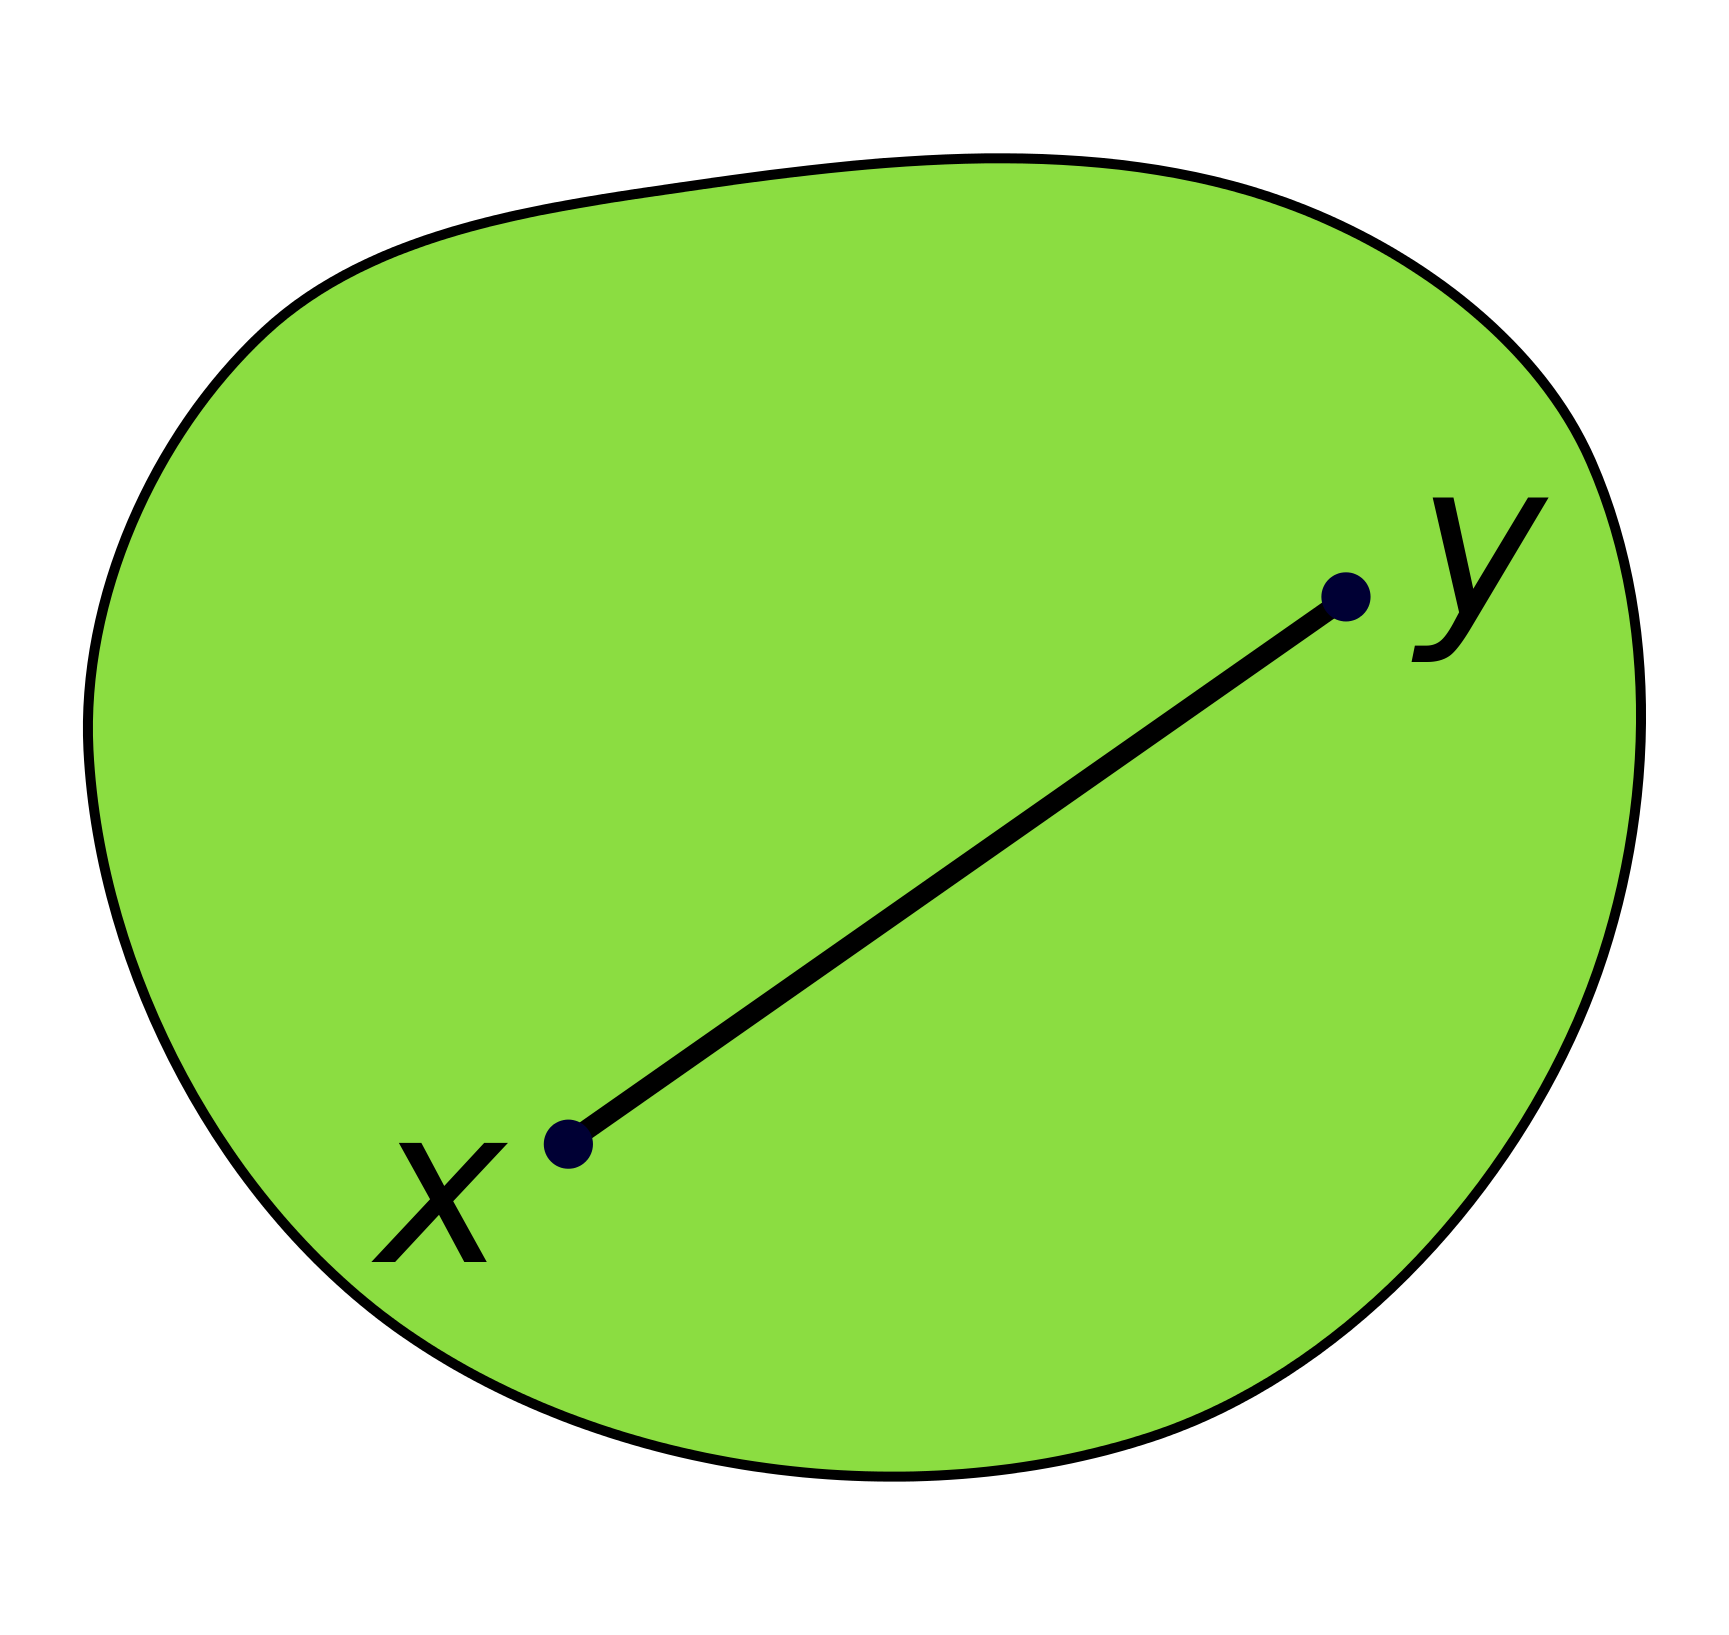
\includegraphics[width=\textwidth]{Convex_polygon_illustration1.png}
	\caption{A convex set}
\end{figure}
\begin{figure}[h]
	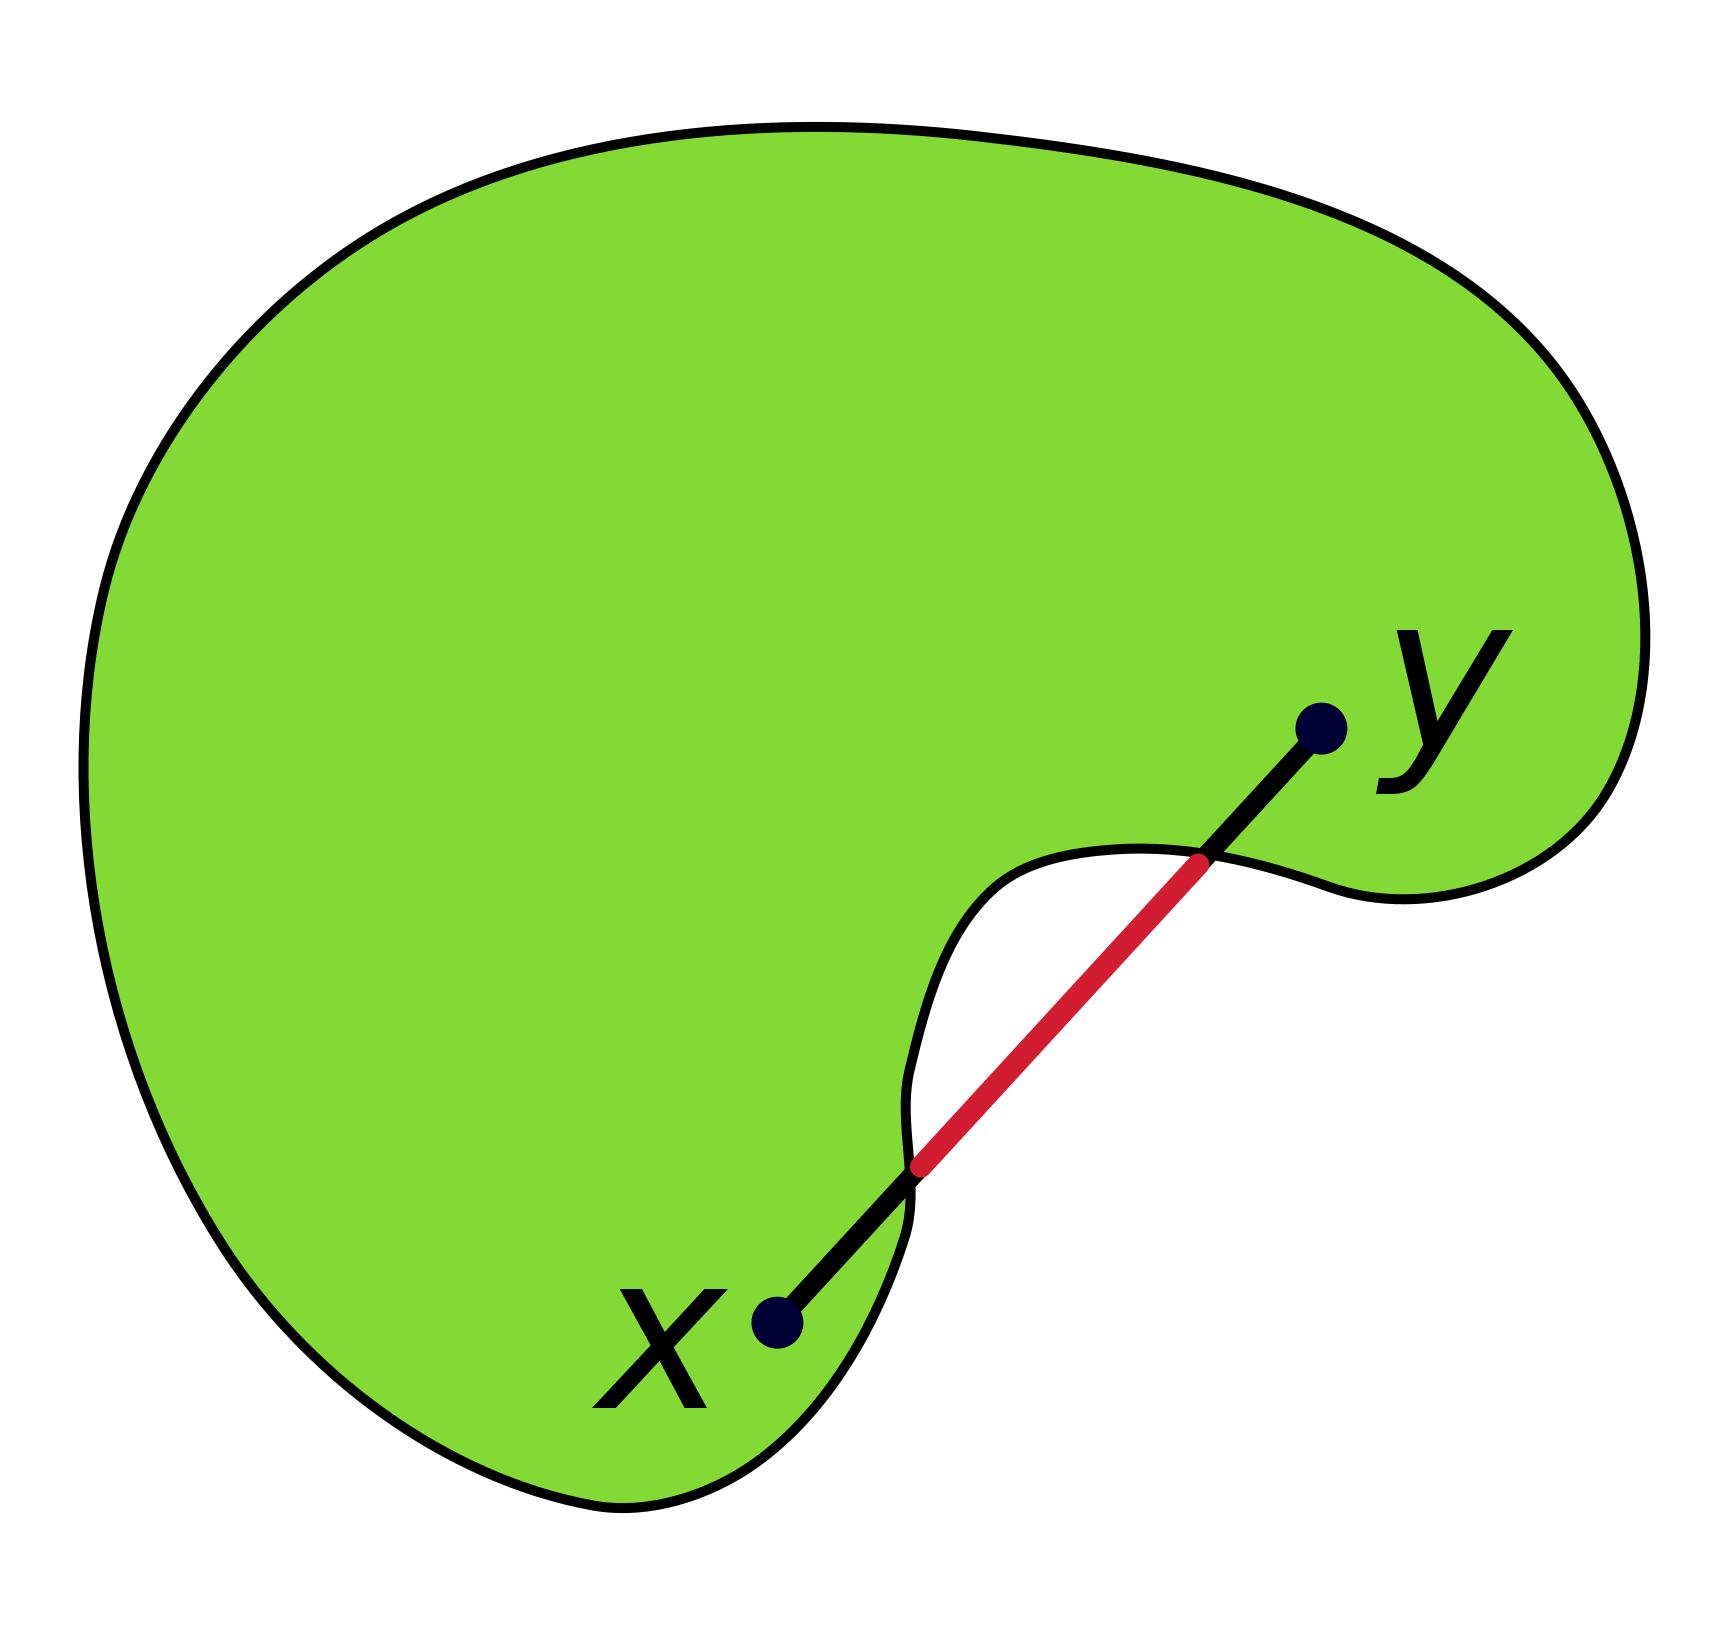
\includegraphics[width=\textwidth]{Convex_polygon_illustration2.png}
	\caption{A non-convex set}	
\end{figure}
\newpage
\begin{Theorem}
	Let $ X $ be an ordered set in the order topology; Let $ Y $ be a subset of $ X $ that is convex in $ X $. Then the order topology on $ Y $ is the same as the topology $ Y $ inherits as a subspace of $ X $.
\end{Theorem}
\begin{proof}
	Consider the ray $ (a,+\infty) $ in $ X $. If $ a \in Y $, its intersection with $ Y $ is
	\begin{equation}
		(a,+\infty)\cap Y =\{x|x\in Y \land x>a \} \nonumber
	\end{equation}
	this is an open ray of the ordered set $ Y $. If $ a \notin Y $, then $ a $ is either a lower bound on $ Y $ or an upper bound on $ Y $ since $ Y $ is convex. In the former case, the set $ (a,+\infty)\cap Y $ equals all of $ Y $; in the latter case, it is empty. \newpara
	A similar argument holds for the intersection of $ (-\infty,a) $ and $ Y $. Since the sets $ (a,+\infty) \cap Y$ and $ (-\infty,a)\cap Y $ form a subbasis for the subspace topology on $ Y $, and since each is open in the order topology, the order topology contains(or is coarser than) the subspace topology. \newpara
	Note that any open ray of $ Y $ equals the intersection of an open ray of $ X $ with $ Y $, so it is open in the subspace topology on $ Y $. Since the open rays of $ Y $ are a subbasis for the order topology on $ Y $, this topology is contained in(or finer than) the subspace topology.
\end{proof}
To avoid ambiguity, if $ X $ is an ordered set in the order topology and $ Y $ is a subset of $ X $, we shall assume that $ Y $ is given the subspace topology unless specified.

\section{Closed Sets and Limit Points}	
\subsection{Closed Sets}
\begin{Theorem}
	Let $ X $ be a topological space. Then the following conditions hold:
	\begin{enumerate}
		\item $ \varnothing $ and $ X $ are closed.
		\item Arbitrary intersections of closed sets are closed.
		\item Finite unions of closed sets are closed.
	\end{enumerate}
\end{Theorem}	
\begin{proof}
	$ (1) $ is obvious. Given a collection of closed sets $ \{A_\alpha \}\alpha \in J $, we have $ X- \bigcap_{\alpha \in J} =\bigcup_{\alpha \in J}(X-A_\alpha)$. Since the set on the right hand side is open, $ \bigcap A_\alpha $ is closed. The third condition can be verified similarly.
\end{proof}
If $ Y $ is a subspace of $ X $, we say that a set $ A $ is \textit{closed in $ Y $} if $ A $ is a subset of $ Y $ and if $ A $ is closed in the subspace topology of $ Y $(that is, if $ Y \setminus A $ is open in $ Y $).
\begin{Theorem}
	Let $ Y $ be a subspace of $ X $. Then a set $ A $ is closed in $ Y $ iff it equals the intersection of a closed set of $ X $ with $ Y $.
\end{Theorem}	
\begin{proof}
	Assume that $ A=C \cap Y $, where $ C $ is closed in $ X $. Then $ X \setminus C $ is open in $ X $, so that $ (X\setminus C)\cap Y $ is open in $ Y $, but then $ (X\setminus C)\cap Y=Y \setminus A $, and hence $ A $ is closed in $ Y $. Conversely, assume that $ A $ is closed in $ Y $. Then $ Y \setminus A $ is open in $ Y $, and by definition it equals the intersection of an open set $ U $ of $ X $ with $ Y $. The set $ X \setminus U $ is closed in $ X $, so $ A=Y\cap (X \setminus U) $, as desired.
\end{proof}
\begin{Theorem}
	Let $ Y $ be a subspace of $ X $. If $ A $ is closed in $ Y $ and $ Y $ is closed in $ X $, then $ A $ is closed in $ X $.
\end{Theorem}	
\subsection{Closure and Interior of a Set}
\begin{Definition}
	Given a subset $ A $ of a topological space $ X $, the \textit{interior} of $ A $ is defined as the union of all open sets contained in $ A $, and the \textit{closure} of $ A $ is defined as the intersection of all closed sets containing $ A $. The interior is denoted by $ \Int A $ and the closure of $ A $ is denoted by $ \Cl A $ or $ \bar{A} $. Obviously $ \Int A $ is open and $ \bar{A} $ is closed. Furthermore
	\begin{equation}
		\Int A \subset A \subset \bar{A} \nonumber
	\end{equation}
	If $ A $ is open, then $ A=\Int A $; if $ A $ is closed, $ A = \bar{A} $.
\end{Definition}
\begin{Theorem}
	Let $ Y $ be a subspace of $ X $; let $ A $ be a subset of $ Y $; let $ \bar{A} $ denote the closure of $ A $ in $ X $. Then the closure of $ A $ in $ Y $ equals $ \bar{A} \cap Y $.
\end{Theorem}
\begin{proof}
	Let $ B $ denote the closure of $ A $ in $ Y $. The set $ \bar{A} $ is closed in $ X $, so $ \bar{A}\cap Y $ is closed. Since $ \bar{A} $ contains $ A $, we have that $ B \subset (\bar{A}\cap Y) $. \newpara
	On the other hand, $ B $ is closed in $ Y $. Hence $ B=C \cap Y $ for some $ C $ closed in $ X $. Then $ C $ is a closed set of $ X $ containing $ A $; because $ \bar{A} $ is the intersection of all such closed sets, we have $ \bar{A} \subset C$. Then $ (\bar{A}\cap Y)\subset (C \cap Y)=B $.
\end{proof}
\begin{Theorem}
	Let $ A $ be a subset of the topological space $ X $.
	\begin{enumerate}
		\item Then $ x \in \bar{A} $ iff every open set $ U $ containing $ x $ intersects $ A $.
		\item Supposing the topology of $ X $ is given by a basis, then $ x \in \bar{A} $ iff every basis element $ B $ containing $ x $ intersects $ A $.
	\end{enumerate}
\end{Theorem}
\begin{proof}
	If $ x \notin \bar{A} $, the set $ U=X\setminus \bar{A} $ is an open set containing $ x $ that does not intersect $ A $. Conversely, if there exists an open set $ U $ containing $ x $ which does not intersect $ A $, then $ X \setminus U $ is a closed set containing $ A $. By the definition of the closure, the set $ X \setminus U $ must contain $ \bar{A} $; therefore, $ x \notin \bar{A} $. The second statement follows from our proof, since any basis element is open.
\end{proof}
\subsection{Limit Points}
\begin{Definition}
	If $ A $ is a subset of the topological space $ X $ and if $ x $ is a point of $ X $, then $ x $ is a \textit{limit point}(or \textit{cluster point} or \textit{point of accumulation}) of $ A $ if every neighborhood of $ x $ intersects $ A $ in some point other than $ x $ itself. Equivalently, $ x $ is a limit point of $ A $ if it belongs to the closure of $ A\setminus{x} $.
\end{Definition}	
\begin{Theorem}
	Let $ A $ be a subset of the topological space $ X $; let $ A^\prime $ be the set of all limit points of $ A $. Then
	\begin{equation}
		\bar{A}=A \cup A^\prime \nonumber
	\end{equation}
\end{Theorem}
\begin{proof}
	If $ x $ is in $ A^\prime $, every neighborhood of $ x $ intersects $ A $. Therefore, $ x $ belongs to $ \bar{A} $. Hence $ A^\prime \subset \bar{A} $. By definition $ A \subset \bar{A} $, and it follows that $ A \cup A^\prime \subset \bar{A} $. \newpara
	Now let $ x $ be a point of $ \bar{A} $. If $ x $ lies in $ A $, the relation $ x \in A \cup A^\prime $ is trivial; suppose that $ x $ is not in $ A $. Since $ x \in \bar{A}$, we know that every neighborhood $ U $ of $ x $ intersects $ A $. Then $ x \in A^\prime $, so that $ x \in A \cup A^\prime $.
\end{proof}
\begin{Corollary}
	A subset of a topological space is closed iff it contains all its limit points.
\end{Corollary}
\section{Hausdorff Spaces}
\begin{Definition}
	A topological space is called a \textit{Hausdorff space} if each pair of points has disjoint neighborhoods.
\end{Definition}	
\begin{Theorem}
	Every finite point set in a Hausdorff space is closed.
\end{Theorem}
\begin{proof}
	It's sufficient to prove that the closure of any one-point set is itself, and this is true since for any point of the complement of this one-point set there exists a neighborhood that does not intersect with the original set.
\end{proof}
\begin{Definition}
	The condition that finite point sets be closed is called the \textit{$ T_1 $ axiom}.
\end{Definition}
\begin{Theorem}
	Let $ X $ be a space satisfying the $ T_1 $ axiom; let $ A $ be a subset of $ X $. Then the point $ x $ is a limit point of $ A $ iff every neighborhood of $ x $ contains infinitely many points of $ A $.
\end{Theorem}
\begin{proof}
	If every neighborhood of a limit point $ x $ only intersects $ A $ at finitely many number of points, then by the $ T_1 $ axiom, any neighborhood of $ x $ is closed, and the complement of any deleted neighborhood of $ x $ is open. Then the intersection of the original neighborhood of $ x $ with this complement is a neighborhood of $ x $, but it does not intersect with $ A $ at all, and this contradicts to the fact that $ x $ is a limit point.
\end{proof}
\begin{Theorem}
	If $ X $ is a Hausdorff space, then a sequence of points of $ X $ converges to at most one point of $ X $.
\end{Theorem}
\begin{proof}
	Suppose that $ x_n $ is a sequence of points of $ X $ that converges to $ x $. If $ y \neq x $, let $ U $ and $ V $ be disjoint neighborhoods of $ x $ and $ y $, respectively. Since $ U $ contains $ x_n $ for all but a finitely many values of $ n $, the set $ V $ cannot. Then $ x_n $ cannot converge to $ y $.
\end{proof}
\begin{Theorem}
	Every simply ordered set is a Hausdorff space in the order topology. The product of two Hausdorff spaces is a Hausdorff space. A subspace of a Hausdorff space is a Hausdorff space.
\end{Theorem}
\begin{proof}
	The first two statements can be verified easily. For any pair of points of this subspace, one can choose two disjoint neighborhoods, and thus their intersection with this subspace are disjoint neighborhoods of this two points respectively in the subspace, but since the subspace topology is just the intersection of open sets in the original topological space with the subspace, we had done selecting two disjoint neighborhoods of two points in the subspace topology.
\end{proof}
\section{Continuous Functions}
\subsection{Continuity of a Function}
\begin{Definition}
	Let $ X $ and $ Y $ be topological spaces. A function $ f:X \to Y $ is said to be \textit{continuous} if for each open subset $ V $ of $ Y $, the set $ f^{-1}(V) $ is an open subset of $ X $. If the topology of $ Y $ is given by a basis $ \mathscr{B} $, then to prove continuity of $ f $ it suffices to show that the inverse image of every basis element is open, since any arbitrary open set of $ Y $ can be written as a union of basis elements. If the topology $ Y $ is given by a subbasis $ \mathscr{S} $, to prove continuity of $ f $ it will suffice to show that the inverse image of each subbasis element is open, since the arbitrary basis element of $ Y $ can be written as a finite intersection of subbasis elements.
\end{Definition}
\begin{Theorem}
	Let $ X $ and $ Y $ be topological spaces; let $ f:X \to Y $. Then the following are equivalent:
	\begin{enumerate}
		\item $ f $ is continuous.
		\item For every subset $ A $ of $ X $, one has $ f(\bar{A})\subset \overline{f(A)}$.
		\item For every closed set $ B $ of $ Y $, the set $ f^{-1}(B) $ is closed in $ X $.
		\item For each $ x \in X $ and each neighborhood $ V $ of $ f(x) $, there is a neighborhood $ U $ of $ x $ such that $ f(U)\subset(V) $.
	\end{enumerate}
If condition $ (4) $ holds for the point $ x $ of $ X $, we say that $ f $ is \textit{continuous at the point $ x $}.
\end{Theorem}
\begin{proof}
	$ (1)\Rightarrow (2) $. Let $ A $ be a subset of $ X $ and $ V $ be a neighborhood of $ f(x) $. Assume that $ x \in \bar{A} $. Then $ f^{-1}(V) $ is an open set of $ X $ containing $ x $; it must intersect $ A  $ in some point $ y $. Then $ V $ intersects $ f(A) $ in the point $ f(y) $, so that $ f(x)\in \overline{f(A)} $, as desired. \newpara
	$ (2)\Rightarrow (3) $. Let $ B $ be closed in $ Y $ and let $ A = f^{-1}(B) $. We have $ f(A)= f(f^{-1}(B))\subset B $. Therefore, if $ x \in \bar{A} $,
	\begin{equation}
		f(x)\in f(\bar{A}) \subset \overline{f(A)}\subset \bar{B} = B \nonumber
	\end{equation}
	so that $ x \in f^{-1}(B)=A $. Thus $ \bar{A} \subset A $, and $ \bar{A} = A $. \newpara
	$ (3)\Rightarrow(1) $. Let $ V $ be an open set of $ Y $. Set $ B=Y\setminus V $. Then
	\begin{equation}
		f^{-1}(B)=f^{-1}(Y)\setminus f^{-1}(V)=X \setminus f^{-1}(V) \nonumber
	\end{equation}
	now $ f^{-1}(B) $ is closed by hypothesis, and $ f^{-1}(V) $ is open in $ X $, as desired.\newpara
	$ (1)\Leftrightarrow(4) $. Let $ x \in X $ and let $ V $ be a neighborhood of $ f(x) $. Then the set $ U=f^{-1}(V) $ is a neighborhood of $ x $ such that $ f(U)\subset V $. Conversely, let $ V $ be an open set of $ Y $; let $ x $ be a point of $ f^{-1}(V) $. Then $ f(x)\in V $, and by hypothesis there is a neighborhood $ U_x $ of $ x $ such that $ f(U_x)\subset V $. Then $ U_x \subset f^{-1}(V)$. It follows that $ f^{-1}(V) $ can be written as the union of the open sets $ U_x $, so that it is open.
\end{proof}
\subsection{Homeomorphisms}
\begin{Definition}
	If a bijection function between two topological spaces and its inverse function are continuous, the original function is called a \textit{homeomorphism}. Equivalently, it means that a homeomorphism is a bijective mapping such that the image of a set is open iff the original set is open. It is analogous with the concept of isomorphism for algebraic structures, which means a homeomorphism preserves the topological structure involved.
\end{Definition}	
\begin{Definition}
	Suppose $ f:X \to Y $ is an injective continuous mapping between two topological spaces. Let $ Z $ be the image set $ f(X) $, considered as a subspace of $ Y $; then the function $ f^\prime:X \to Z $ obtained by restricting the range of $ f $ is bijective. If $ f^\prime $ happens to be a homeomorphism of $ X $ with $ Z $, it is said that the mapping $ f:X \to Y $ is a \textit{topological imbedding}, or an \textit{imbedding}, of $ X $ in $ Y $.
\end{Definition}
\begin{Example}
	The bijective order-preserving correspondence $ F:(1,-1)\to \Real $ defined by
	\begin{equation}
		F(x)=\frac{x}{1-x^2} \nonumber
	\end{equation}
	is a homeomorphism between $ (-1,1) $ with $ \Real $. Its inverse $ G $ is
	\begin{equation}
		G(y)=\frac{2y}{1+(1+4y^2)^{1/2}} \nonumber
	\end{equation}
\end{Example}
\section{Constructing Continuous Functions}
\begin{Theorem}[Rules for Constructing Continuous Functions]
	Let $ X $, $ Y $, and $ Z $ be topological spaces.
	\begin{enumerate}
		\item (Constant function) If $ f:X \to Y $ maps all of $ X $ into the single point $ y_0 $ of $ Y $, then $ f $ is continuous.
		\item (Inclusion) If $ A $ is a subspace of $ X $, the inclusion function $ j:A \to X $ is continuous.
		\item (Composites) If $ f:X \to Y $ and $ g:Y \to Z $ are continuous, then the map $ g \circ f $ is continuous.
		\item (Restricting the domain) If $ f:X \to Y $ is continuous, and if $ A $ is a subspace of $ X $, then the restricted function $ f|_A:A \to Y $ is continuous.
		\item (Restricting or expanding the range) Let $ f:X \to Y $ be continuous. If $ Z $ is a subspace of $ Y $ containing the image set $ f(X) $, then the function $ g:X \to Z $ obtained by restricting the range of $ f $ is continuous. If $ Z $ is a space having $ Y $ as a subspace, then the function $ h:X \to Z $ obtained by expanding the range of $ f $ is continuous.
		\item (Local formulation of continuity) The map $ f:X \to Y $ is continuous if $ X $ can be written as the union of open sets $ U_\alpha $ such that $ f|_{U_\alpha} $ is continuous for each $ \alpha $.
	\end{enumerate}
\end{Theorem}
\begin{proof}
	\begin{enumerate}
		\item Let $ f(x)=y_0 $ for each $ x \in X $ and let $ V $ be open in $ Y $. The set $ f^{-1}(V) $ equals $ X $ or $ \varnothing $, depending on whether $ V $ contains $ y_0 $ or not. In either case, it is open.
		\item If $ U $ is open in $ X $, then $ j^{-1}(U)=U\cap A $, which is open in $ A $.
		\item If $ U $ is open in $ Z $, then $ g^{-1}(U) $ is open in $ Y $ and $ f^{-1}(g^{-1}(U)) $ is open in $ X $, but
		\begin{equation}
			f^{-1}(g^{-1}(U)) =(g \circ f)^{-1}(U) \nonumber
		\end{equation}
		\item The function $ f|_A$ equals the composite of the inclusion mapping $ j:A \to X $ and the mapping $ f:X \to Y $, both of which are continuous.
		\item Let $ f:X \to Y $ be continuous. If $ f(X)\subset Z \subset Y $, we show that the function $ g:X \to Z $ obtained from $ f $ is continuous. Let $ B $ be open in $ Z $. Then $ B=Z \cap U $ for some open set $ U $ of $ Y $. Because $ Z $ contains the entire image set $ f(X) $,
		\begin{equation}
			f^{-1}(U)=g^{-1}(B)\nonumber
		\end{equation}
		Since the left side is open by the definition of continuity, so is $ g^{-1}(B) $.\\
		To show $ h:X \to Z $ is continuous if $ Z $ has $ Y $ as a subspace, note that $ h $ is the composition of the mapping $ f:X \to Y $ and the inclusion map $ j:Y \to Z $.
		\item By hypothesis, we can write $ X $ as a union of open sets $ U_\alpha $, such that $ f|_{U_\alpha} $, is continuous for each $ \alpha $. Let $ V $ be an open set in $ Y $. Then
		\begin{equation}
			f^{-1}(V)\cap U_\alpha = (f|_{U_\alpha})^{-1}(V) \nonumber
		\end{equation}
		because both expressions represent the set of those points $ x $ lying in $ U_\alpha $ for which $ f(x)\in V $. Since $ f|_U $ is continuous, this set is open in $ U_\alpha $, and hence open in $ X $. But
		\begin{equation}
			f^{-1}(V)=\bigcup_{\alpha}(f^{-1}(V)\cap U_\alpha) \nonumber
		\end{equation}
		so that $ f^{-1}(V) $ is also open in $ X $.
	\end{enumerate}
\end{proof}	
\begin{Theorem}[The pasting lemma]
	Let $ X = A \cup B $, where $ A $ and $ B $ are closed in $ X $. Let $ f:A \to Y $ and $ g:B \to Y $ be continuous. If $ f(x)=g(x) $ for every $ x \in A \cap B $, then $ f $ and $ g $ combine to give a continuous function $ h:X \to Y $, defined by setting $ h(x)=f(x) $ if $ x \in A $, and $ h(x)=g(x) $ if $ x \in B $.
\end{Theorem}
\begin{proof}
	Let $ C $ be a closed subset of $ Y $. Now
	\begin{equation}
		h^{-1}(C)=f^{-1}(C)\cup g^{-1}(C) \nonumber
	\end{equation}
	The fact that $ f $ and $ g $ are continuous make each term of the right-hand side closed in their respectively domain, and hence they are closed in $ X $, which makes $ h^{-1}(C) $ closed in $ X $.
\end{proof}
\begin{Theorem}[Maps into products]
	Let $ f:A \to X \times Y $ given by the equation
	\begin{equation}
		f(a)=(f_1(a),f_2(a))\nonumber
	\end{equation}
	Then $ f $ is continuous iff the functions $ f_1 $ and $ f_2 $ are continuous.
\end{Theorem}
The mapping $ f_1 $ and $ f_2 $ are called the \textit{coordinate functions} of $ f $.
\begin{proof}
	Let $ \pi_1:X \times Y \to X $ and $ \pi_2 :X \times Y \to Y $ be projections onto the first and second factors, respectively. These maps are continuous. For $ \pi_1^{-1}(U)=U \times Y $ and $ \pi_2^{-1}(V)=X \times V $, and these sets are open iff $ U $ and $ V $ are open. Note that for each $ a \in A$
	\begin{equation}
		f_1(a)=\pi_1(f(a))\quad \text{and}\quad f_2(a)=\pi_2(f(a)) \nonumber
	\end{equation}
	If $ f $ is continuous, then $ f_1 $ and $ f_2 $ are composition of continuous functions and therefore continuous. Conversely, suppose that $ f_1 $ and $ f_2 $ are continuous. We show that for each basis element $ U \times V $ for the topology of $ X \times Y $, its inverse image $ f^{-1}(U \times V) $ is open. A point $ a $ is in $ f^{-1}(U \times V) $ iff $ f(a)\in U \times V $, therefore
	\begin{equation}
		f^{-1}(U \times V) = f_1^{-1}(U)\cap f_2^{-1}(V)\nonumber
	\end{equation}
	Since both terms of the right-hand side are open, so is their intersection.
\end{proof}
\section{The Product Topology}	
\begin{Definition}
	Let $ J $ be an index set. Given a set $ X $, we define a \textit{$ J $-tuple} of elements of $ X $ to be a function $ x:J \to X $. If $ \alpha $ is an element of $ J $, the value of $ x $ at $ \alpha $ is usually denoted by $ x_\alpha $ and called the $ \alpha $th \textit{coordinate} of $ x $. The function $ x $ itself is denoted by
	\begin{equation}
		(x_\alpha)_{\alpha \in J} \nonumber
	\end{equation}
	The set of all $ J $-tuples of elements of $ X $ is denoted by $ X^J $.
\end{Definition}
\begin{Definition}
	Let $ \{A_\alpha \}_{\alpha \in J} $ be an indexed family of sets; let $ X=\bigcup_{\alpha \in J}A_\alpha $. The \textit{cartesian product} of this indexed family, denoted by
	\begin{equation}
		\prod_{\alpha \in J}A_\alpha \nonumber
	\end{equation}
	is defined to be the set of all $ J $-tuples $ (x_\alpha)_{\alpha \in J} $ of elements of $ X $ such that $ x_\alpha \in A_\alpha $ for each $ \alpha \in J $. That is, it is the set of all functions
	\begin{equation}
		x:J \to \bigcup_{\alpha \in J}A_\alpha \nonumber
	\end{equation}
	such that $ x(\alpha)\in A_\alpha $ for each $ \alpha \in J $.
\end{Definition}
\begin{Definition}
	Let $ \{X_\alpha \}_{\alpha \in J} $ be an indexed family of topological spaces. Let us take as a basis for a topology on the product space
	\begin{equation}
		\prod_{\alpha \in J}X_\alpha \nonumber
	\end{equation}
	the collection of all sets of the form
	\begin{equation}
		\prod_{\alpha \in J}U_\alpha \nonumber
	\end{equation}
	where $ U_\alpha $ is open in $ X_\alpha $. The topology generated by this basis is called the \textit{box topology}.
\end{Definition}	
\begin{Definition}
	The \textit{projection mapping} associated with the index $ \beta $ is defined as a function assigning to each element of the product space its $ \beta $th coordinate.
	\begin{equation}
		\pi_\beta:\prod_{\alpha \in J}X_\alpha \to X_\beta ,\quad \pi_\beta((x_\alpha)_{\alpha \in J}) = x_\beta \nonumber
	\end{equation}
\end{Definition}	
\begin{Definition}
	Let $ \mathscr{S}_\beta $ denote the collection
	\begin{equation}
		\mathscr{S}_\beta = \{\pi_\beta^{-1}(U_\beta)|U_\beta \text{ open in }X_\beta \} \nonumber
	\end{equation}
	and let $ \mathscr{S} $ denote the union of these collections,
	\begin{equation}
		\mathscr{S}=\bigcup_{\beta \in J}\mathscr{S}_\beta \nonumber
	\end{equation}
	The topology generated by the subbasis $ \mathscr{S} $ is called the \textit{product topology}. In this topology $ \prod_{\alpha \in J}X_\alpha $ is called a \textit{product space}.
\end{Definition}
\begin{Theorem}[Comparison of the Box and Product Topologies]
	The boc topology on $ \prod X_\alpha $ has as basis all sets of the form $ \prod U_\alpha $, where $ U_\alpha $ is open in $ X_\alpha $ for each $ \alpha $. The product topology on $ \prod X_\alpha $ has as basis all sets of the form $ \Pi U_\alpha $, where $ U_\alpha $ is open in $ X_\alpha $ for each $ \alpha $ and $ U_\alpha $ equals $ X_\alpha $ except for finitely many values of $ \alpha $.
\end{Theorem}
For finite products $ \prod_{\alpha =1}^{n}X_\alpha $ the two topologies are the same. Generally the box topology is finer than the product topology.
\begin{Theorem}
	Suppose the topology on each space $ X_\alpha $ is given by a basis $ \mathscr{B}_\alpha $. The collection of all sets of the form
	\begin{equation}
		\prod_{\alpha \in J}B_\alpha \nonumber
	\end{equation}
	where $ B_\alpha \in \mathscr{B}_\alpha $ for each $ \alpha $, will serve as a basis for the box topology on $ \prod_{\alpha \in J}X_\alpha $.\newpara
	The collection of all sets of the same form, where $ B_\alpha \in \mathscr{B}_\alpha $ for finitely many indices $ \alpha $ and $ B_\alpha = X_\alpha $ for all the remaining indices, will serve as a basis for the product topology $ \prod_{\alpha \in J}X_\alpha $.
\end{Theorem}	
\begin{proof}
	\exercise
\end{proof}
\begin{Theorem}
	Let $ A_\alpha $ be a subspace of $ X_\alpha $, for each $ \alpha \in J $. Then $ \prod A_\alpha $ is a subspace of $ \prod X_\alpha $ if both products are given the box topology, or if both products are given the product topology.
\end{Theorem}
\begin{proof}
	\exercise
\end{proof}
\begin{Theorem}
	If each space $ X_\alpha $ is Hausdorff space, then $ \prod X_\alpha $ is a Hausdorff space in both the box and product topologies.
\end{Theorem}
\begin{proof}
	\exercise
\end{proof}
\begin{Theorem}
	Let $ \{X_\alpha \} $ be an indexed family of spaces; let $ A_\alpha \subset X_\alpha$ for each $ \alpha $. If $ \prod X_\alpha $ is given either the product or the box topology, then
	\begin{equation}
		\prod \bar{A}_\alpha = \overline{\prod A_\alpha} \nonumber
	\end{equation}
\end{Theorem}
\begin{proof}
	Let $ x=(x_\alpha) $ be a point of $ \prod \bar{A}_\alpha $; we show that $ x \in \overline{\prod A_\alpha} $. Let $ U = \prod U_\alpha $ be a basis element for either the box or product topology that contains $ x $. Since $ x_\alpha \in \bar{A}_\alpha$, we can choose a point $ y_\alpha \in U_\alpha \cap A_\alpha $ for each $ \alpha $. Then $ y=(y_\alpha) $ belongs to both $ U $ and $ \prod A_\alpha $. Since $ U $ is arbitrary, it follows that $ x $ belongs to the closure of $ \prod A_\alpha $. \newpara
	Conversely, suppose $ x=(x_\alpha) $ lies in the closure of $ \prod A_\alpha $, in either topology. We show that for any given index $ \beta $, we have $ x_\beta \in \bar{A}_\beta $. Let $ V_\beta $ be an arbitrary open set of $ X_\beta $ containing $ x_\beta $. Since $ \pi_\beta^{-1}(V_\beta) $ is open in $ \prod X_\alpha $ in either topology, it contains a point $ y=(y_\alpha) $ if $ \prod A_\alpha $. Then $ y_\beta $ belongs to $ V_\beta \cap A_\beta $. It follows that $ x_\beta \in \bar{A}_\beta $.
\end{proof}
\begin{Theorem}
	Let $ f:A \to \prod_{\alpha \in J}X_\alpha $ be given by the equation
	\begin{equation}
		f(a)=(f_\alpha(a))_{\alpha \in J} \nonumber
	\end{equation}
	where $ f_\alpha :A \to X_\alpha$ for each $ \alpha $. Let $ \prod X_\alpha $ have the product topology. Then the function $ f $ is continuous iff each function $ f_\alpha $ is continuous.
\end{Theorem}	
\begin{proof}
	Let $ \pi_\beta $ be the projection of the product onto its $ \beta $th factor. The function $ \pi_\beta $ is continuous, for if $ U_\beta $ is open in $ X_\beta $, the set $ \pi_{\beta}^{-1}(U_\beta) $ is a subbasis element for the product topology on $ X_\alpha $. Now suppose that $ f:A \to \prod X_\alpha $ is continuous. The function $ f_\beta $ equals the composite $ \pi_\beta \circ f $; being the composite of two continuous functions, it is continuous. \newpara
	Conversely, suppose that each coordinate function $ f_\alpha $ is continuous. To prove that $ f $ is continuous, it suffices to prove that the inverse image under $ f $ of each subbasis element is open in $ A $; A typical subbasis element for the product topology on $ \prod X_\alpha $ is a set of the form $ \pi_\beta^{-1}(U_\beta) $, where $ \beta $ is some index and $ U_\beta $ is open in $ X_\beta $. Now
	\begin{equation}
		f^{-1}(\pi_\beta^{-1}(U_\beta))=f^{-1}_\beta (U_\beta) \nonumber
	\end{equation}
	because $ f_\beta = \pi_\beta \circ f $. Since $ f_\beta $ is continuous, this set is open in $ A $, as desired.
\end{proof}
The theorem only holds on product topology, and we'll present a counterexample below.
\begin{Example}
	Consider $ \Real^\omega $, the countably infinite product of $ \Real $ with itself. Recall that
	\begin{equation}
		\Real^\omega = \prod_{n\in \Zahlen_+} X_n \nonumber
	\end{equation}
	where $ X_n=\Real $ for each $ n $. Let us defined a function $ f:\Real \to \Real^\omega $ by the equation
	\begin{equation}
		f(t)=(t,t,t,\cdots)\nonumber
	\end{equation}
	the $ n $th coordinate function of $ f $ is the function $ f_n(t)=t $. Each of the coordinate functions is continuous; therefore, the function $ f $ is continuous if given the product topology. But $ f $ is not continuous if $ \Real^\omega $ is given the box topology. Consider, for example. the basis element
	\begin{equation}
		B=(-1,1)\times (-\frac{1}{2},\frac{1}{2})\times (-\frac{1}{3},\frac{1}{3})\times \cdots \nonumber
	\end{equation}
	for the box topology. We assert that $ f^{-1}(B) $ is not open in $ \Real $. If $ f^{-1}(B) $ were open in $ \Real $, it would contain some interval $ (-\delta,\delta) $ about the point $ 0 $. This would mean that $ f((-\delta,\delta))\subset B $, so that, applying $ \pi_n $ to both sides of the inclusion,
	\begin{equation}
		f_n((-\delta,\delta))=(-\delta,\delta)\subset (-1/n,1/n) \nonumber
	\end{equation}
	for all $ n $, a contradiction.
\end{Example}

\section{The Metric Topology}	
\begin{Definition}
	A \textit{metric} on a set $ X $ is a function
	\begin{equation}
		d:X \times X \to \Real \nonumber
	\end{equation}
	having the following properties:
	\begin{enumerate}
		\item $ d(x,y)\geqslant 0 $ for all $ x,y \in X $; equality holds iff $ x=y $.
		\item $ d(x,y)=d(y,x) $ for all $ x,y \in X $.
		\item (Triangle inequality) $ d(x,y)+d(y,z)\geqslant d(x,z) $, for all $ x,y,z \in X $.
	\end{enumerate}
Given a metric $ d $ on $ X $, the number $ d(x,y) $ is often called the \textit{distance} between $ x $ and $ y $ in the metric $ d $.
\end{Definition}	
\begin{Definition}
	If $ d $ is a metric on the set $ X $, then the collection of all $ \varepsilon $-balls $ B_d(x,\varepsilon) $, for $ x \in X $ and $ \varepsilon >0$, is a basis for a topology on $ X $, called the \textit{metric topology} induced by $ d $.
\end{Definition}
	
\begin{Definition}
	If $ X $ is a topological space, $ X $ is said to be \textit{metrizable} if there exists a metric $ d $ on the set $ X $ that induces the topology of $ X $. A \textit{metric space} is a metrizable space $ X $ together with a specific metric $ d $ that gives the topology of $ X $.
\end{Definition}	
\begin{Definition}
	Let $ X $ be a metric space with metric $ d $. A subset $ A $ of $ X $ is said to be \textit{bounded} if there is some number $ M $ such that
	\begin{equation}
		d(a_1,a_2)\leqslant M \nonumber
	\end{equation}
	for every pair $ a_1,a_2 $ of points of $ A $. If $ A $ is bounded and nonempty, the \textit{diameter} of $ A $ is defined to be the number
	\begin{equation}
		d(A)=\sup \{d(a_1,a_2)|a_1,a_2 \in A \} \nonumber
	\end{equation}
\end{Definition}
\begin{Theorem}
	Let $ X $ be a metric space with metric $ d $. Define $ \bar{d}:X \times X \to \Real $ by the equation
	\begin{equation}
		\bar{d}(x,y)=\min \{d(x,y),1 \} \nonumber
	\end{equation}
	Then $ \bar{d} $ is a metric that induces the same topology as $ d $ and called the \textit{standard bounded metric} corresponding to $ d $.
\end{Theorem}
\begin{proof}
	We only need to check the triangle equality for $ \bar{d} $, and check the case either $ d(x,y)\geqslant 1 $ or $ d(y,z)\geqslant 1 $ as well as $ d(x,y)<1 $ and $ d(y,z)<1 $. Now we note that in any metric space, the collection $ \varepsilon $-balls with $ \varepsilon<1 $ forms a basis for the metric topology, for every basis element containing $ x $ contains such an $ \varepsilon $-ball centered at $ x $. It follows that $ d $ and $ \bar{d} $ induce the same topology on $ X $, because the collection of $ \varepsilon $-balls with $ \varepsilon<1 $ under these two metrices are the same collection.
\end{proof}
\begin{Definition}
	Given $ \vec{x}=(x_1,\cdots,x_n) $ in $ \Real^n $, we define the \textit{norm} of $ \vec{x} $ by the equation
	\begin{equation}
		\norm{\vec{x}} = (x_1^2+\cdots +x_n^2)^{1/2} \nonumber
	\end{equation}
	and we define the \textit{euclidean metric} $ d $ on $ \Real^n $ by the equation
	\begin{equation}
		d(\vec{x},\vec{y})=\norm{\vec{x}-\vec{y}} \nonumber
	\end{equation}
	We define the \textit{square metric} $ \rho $ by the equation
	\begin{equation}
		\rho(\vec{x},\vec{y}) = \max \{|x_1-y_1|,\cdots, |x_n-y_n|\} \nonumber
	\end{equation}
\end{Definition}	
\begin{Lemma}
	Let $ d $ and $ d^\prime $ be two metrices on the set $ X $; let $ \mathscr{T} $ and $ \mathscr{T}^\prime $ be the topology they induce, respectively. Then $ \mathscr{T}^\prime $ is finer than $ \mathscr{T} $ iff for each $ x \in X $ and each $ \varepsilon>0 $, there exists a $ \delta >0 $ such that
	\begin{equation}
		B_{d^\prime}(x,\delta) \subset B_{d}(x,\varepsilon) \nonumber
	\end{equation}
\end{Lemma}
\begin{Theorem}
	The topologies on $ \Real^n $ induced by the euclidean metric $ d $ and the square metric $ \rho $ are the same as the product topology on $ \Real^n $.
\end{Theorem}
\begin{proof}
	Let $ \vec{x} $ and $ \vec{y} $ be two points of $ \Real^nn  $. It is easy to check that
	\begin{equation}
		\rho(\vec{x},\vec{y})\leqslant d(\vec{x},\vec{y}) \leqslant \sqrt{n} \rho(\vec{x},\vec{y}) \nonumber
	\end{equation}
	The first inequality shows that $ B_d(\vec{x},\varepsilon) \subset B_\rho(\vec{x},\varepsilon)$ for all $ \vec{x} $ and $ \varepsilon $. Similarly, the second inequality snows that $ B_\rho (\vec{x},\varepsilon/\sqrt{n}) \subset B_d(\vec{x},\varepsilon)$,and then the two metric topologies are the same. \newpara
	Now we show that the product topology is the same as that given by the metric $ \rho $. First, let
	\begin{equation}
		B=(a_1,b_1)\times \cdots \times (a_n,b_n) \nonumber
	\end{equation}
	be a basis element for the product topology, and $ \vec{x}=(x_1,\cdots,x_n) $ be an element of $ B $. For each $ i $, there is an $ \varepsilon_i $ such that
	\begin{equation}
		(x_i-\varepsilon_i,x_i+\varepsilon_i)\subset (a_i,b_i) \nonumber
	\end{equation}
	choose $ \varepsilon = \min \{\varepsilon_1,\cdots,\varepsilon_n \} $. Then $ B_\rho(\vec{x},\varepsilon)\subset B $. As a result, the $ \rho $-topology is finer than the product topology. \newpara
	Conversely, let $ B_\rho(\vec{x},\varepsilon) $ be a basis element for the $ \rho $-topology. Given the element $ \vec{y}\in B_\rho(\vec{x},\varepsilon) $, we need to find a basis element $ B $ for the product topology such that
	\begin{equation}
		\vec{y}\in B \subset B_\rho(\vec{x},\varepsilon) \nonumber
	\end{equation}
	But this is trivial, for
	\begin{equation}
		B_\rho(\vec{x},\varepsilon)=(x_1-\varepsilon,x_1+\varepsilon)\times \cdots \times  (x_n-\varepsilon,x_n+\varepsilon) \nonumber
	\end{equation}
	is itself a basis element for the product topology.
\end{proof}	
\begin{Definition}
	Given an index set $ J $, and given points $ \vec{x}=(x_\alpha)_{\alpha \in J} $ and $ \vec{y}=(y_\alpha)_{\alpha \in J}$ of $ \Real^J $, let us define a metric $ \bar{\rho} $ on $ \Real^J $ by the equation
	\begin{equation}
		\bar{\rho}(\vec{x},\vec{y})=\sup \{\bar{d}(x_\alpha,y_\alpha)|\alpha \in J \}
	\end{equation}
	where $ \bar{d} $ is the standard bounded metric on $ \Real $. The metric $ \bar{\rho} $ is called the \textit{uniform metric} on $ \Real^J $, and the topology it induces is called the \textit{uniform topology}.
\end{Definition}
\begin{Theorem}
	The uniform topology on $ \Real^J $ is finer than the product topology and coarser than the box topology; these three topologies are all different if $ J $ is infinite.
\end{Theorem}
\begin{proof}
Suppose that we are given a point $ \vec{x} =(x_\alpha)_{\alpha \in J}$ and a product topology basis element $ \prod U_\alpha $ about $ \vec{x} $. Let $ \alpha_1,\cdots,\alpha_n $ be the indices for which $ U_\alpha \neq \Real $. Then for each $ i $, choose $ \varepsilon_i >0 $ so that the $ \varepsilon_i $-ball centered at $ x_\alpha $ in the $ \bar{d} $ matrix is contained in $ U_{\alpha_i} $; this is possible because $ U_{\alpha_i} $ is open in $ \Real $. Let $ \varepsilon=\min \{\varepsilon_1,\cdots,\varepsilon_n \} $; then the $ \varepsilon $-ball centered at $ \bar{\rho} $ metric is contained in $ \prod U_\alpha $. For if $ \vec{z} $ is a point of $ \Real^J $ such that $ \bar{\rho}(\vec{x},\vec{z})<\varepsilon $, then $ \bar{d}(\vec{x},\vec{z})<\varepsilon $ for all $ \alpha $, so that $ \vec{z}\in \prod U_\alpha $. It follows that the uniform topology is finer than the product topology. These two topologies are different since any point in a open set in the uniform topology does not have a neighborhood in the product topology that is contained in this open set(any neighborhood in the product topology is unbounded).   \newpara

On the other hand, let $ B $ be the $ \varepsilon $-ball centered at $ \vec{x} $ in the $ \bar{\rho} $ metric. Then the box neighborhood
\begin{equation}
	U=\prod (x_\alpha - \frac{1}{2}\varepsilon,x_\alpha + \frac{1}{2}\varepsilon) \nonumber
\end{equation}
of $ \vec{x} $ is contained in $ B $. For if $ \vec{y}\in U $, then $ \bar{d}(x_\alpha,y_\alpha)<\frac{1}{2}\varepsilon $ for all $ \alpha $, so that $ \bar{\rho}(\vec{x},\vec{y})\leqslant \frac{1}{2}\varepsilon $. Now consider the $ \varepsilon $-ball in the box topology for the point $ \vec{x} $. Clearly it is open in the box topology, but it's not open in the uniform topology, for the point $ (x_1+\varepsilon/2,x_2+2\varepsilon/3,x_3+3\varepsilon/4,\cdots) $ does not have any neighborhood that is contained in the previously mentioned $ \varepsilon $-ball in the uniform topology.\newpara

\end{proof}
\begin{Theorem}
	Let $ \bar{d}(a,b)=\min \{|a-b|,1 \} $ be the standard bounded metric on $ \Real $. If $ \vec{x} $ and $ \vec{y} $ are two points of $ \Real^\omega $, define
	\begin{equation}
		D(\vec{x},\vec{y}) =\sup \{ \frac{\bar{d}(x_i,y_i)}{i}\} \nonumber
	\end{equation}
	Then $ D $ is a metric that induces the product topology on $ \Real^\omega $.
\end{Theorem}
\begin{proof}
	The properties of a metric are satisfied trivially except for the triangle inequality, which is proved by noting that for all $ i $,
	\begin{equation}
		\frac{\bar{d}(x_i,z_i)}{i}\leqslant \frac{\bar{d}(x_i,y_i)}{i}+	\frac{\bar{d}(y_i,z_i)}{i} \leqslant D(\vec{x},\vec{y})+D(\vec{y},\vec{z}) \nonumber
	\end{equation}
	so that
	\begin{equation}
		\sup \{\frac{\bar{d}(x_i,z_i)}{i} \}\leqslant D(\vec{x},\vec{y})+D(\vec{y},\vec{z}) \nonumber
	\end{equation}
	
	Now we prove that $ D $ gives the product topology. First, let $ U $ be open in the metric topology and let $ \vec{x}\in U $; we find an open set $ V $ in the product topology such that $ \vec{x}\in V \subset U $. Choose an $ \varepsilon $-ball $ B_D(\vec{x},\varepsilon) $ lying in $ U $. Then choose $ N $ large enough that $ 1/N < \varepsilon $. Finally, let $ V $ be the basis element for the product topology
	\begin{equation}
		V=(x_1-\varepsilon,x_1+\varepsilon)\times \cdots \times (x_N-\varepsilon,x_N+\varepsilon)\times \Real \times \Real \times \cdots \nonumber
	\end{equation}
	We assert that $ V \subset B_D(\vec{x}\varepsilon) $: Given any $ \vec{y}\in\Real^\omega $,
	\begin{equation}
		\frac{\bar{d}(x_i,y_i)}{i}\leqslant \frac{1}{N} \quad \text{for}\quad i \geqslant N \nonumber
	\end{equation}
	Therefore,
	\begin{equation}
		D(\vec{x},\vec{y})\leqslant \max\{\frac{\bar{d}(x_1,y_1)}{1},\cdots,\frac{\bar{d}(x_N,y_N)}{N},\frac{1}{N} \} \nonumber
	\end{equation}
	If $ \vec{y} $ is in $ V $, this expression is less than $ \varepsilon $, so that $ V \subset B_D(\vec{x},\varepsilon) $, as desired. \newpara
	Conversely, consider a basis element
	\begin{equation}
		U=\prod_{i\in \Zahlen_+}U_i \nonumber
	\end{equation}
	for the product topology, where $ U_i $ is open in $ \Real $ for $ i=\alpha_1,\cdots,\alpha_n $ and $ U_i=\Real $ for all other indices $ i $. Given $ \vec{x}\in U $, we find an open set $ V $ of the metric topology such that $ \vec{x}\in V \subset U $. Choose an interval $ (x_i-\varepsilon_i,x_i+\varepsilon_i) $ in $ \Real $ centered about $ x_i $ and lying in $ U_i $ for $ i=\alpha_1,\cdots,\alpha_n $; choose each $ \varepsilon_i \leqslant 1 $. Then define
	\begin{equation}
		\varepsilon=\min\{\varepsilon_i/i|i=\alpha_1,\cdots,\alpha_n \} \nonumber
	\end{equation}
	We assert that
	\begin{equation}
		\vec{x}\in B_D(\vec{x},\varepsilon)\subset U \nonumber
	\end{equation}
	Let $ \vec{y} $ be a point of $ B_D(\vec{x},\varepsilon) $. Then for all $ i $,
	\begin{equation}
		\frac{\bar{d}(x_i,y_i)}{i}\leqslant D(\vec{x},\vec{y}) < \varepsilon \nonumber
	\end{equation}
	Now if $ i=\alpha_1,\cdots,\alpha_n $, then $ \varepsilon \leqslant \varepsilon_i/i $, so that $ \bar{d}(x_i,y_i)<\varepsilon_i \leqslant 1 $; it follows that $ |x_i-y_i|<\varepsilon_i $. Therefore, $ \vec{y}\in \prod U_i $, as desired.
\end{proof}
\begin{Proposition}
	If $ A $ is a subspace of the topological space $ X $ and $ d $ is a metric for $ X $, then the restriction of $ d $ to $ A \times A $ is a metric for the topology of $ A $.
\end{Proposition}
The Hausdorff axiom is satisfied by every metric topology. If $ x $ and $ y $ are distinct points of the metric space $ (X,d) $, we let $ \varepsilon = \frac{1}{2}d(x,y) $; then the triangle inequality implies that $ B_d(x,\varepsilon) $ and $ B_d(y,\varepsilon) $ are disjoint. \newpara
In general, countable products of metrizable spaces are metrizable;
\begin{proof}
	\exercise
\end{proof}
\begin{Lemma}[The Sequence Lemma]
	Let $ X $ be a topological space; let $ A \subset X $. If there is a sequence of points of $ A $ converging to $ x $, then $ x \in \bar{A} $; the converse holds if $ X $ is metrizable.
\end{Lemma}
\begin{proof}
	Suppose that $ x_n \to x $, where $ x_n \in A $. Then every neighborhood of $ x $ contains a point of $ A $, so $ x \in \bar{A} $. Conversely, suppose that $ X $ is metrizable and $ x \in \bar{A} $. Let $ d $ be a metric for the topology of $ X $. For each positive integer $ n $, take the neighborhood $ B_d(x,1/n) $ of $ x $, and choose $ x_n $ to be a point of its intersection with $ A $. Then any open set $ U $ containing $ x $ contains an $ \varepsilon $-ball centered at $ x $; if we choose $ N $ so that $ 1/N<\varepsilon $, then $ U $ contains $ x_i $ for all $ i\geqslant N $.
\end{proof}
\begin{Theorem}
	Let $ f:X \to Y $. If the function $ f $ is continuous, then for every convergent sequence $ x_n \to x $ in $ X $, the sequence $ f(x_n) $ converges to $ f(x) $. The converse holds if $ X $ is metrizable.
\end{Theorem}
\begin{proof}
	Assume that $ f $ is continuous. Given $ x_n \to x $, we wish to show that $ f(x_n)\to f(x) $. Let $ V $ be a neighborhood of $ f(x) $. Then $ f^{-1}(V) $ is a neighborhood of $ x $, and so there is an $ N $ such that $ x_n \in f^{-1}(V) $ for $ n \geqslant N $. Then $ f(x_n)\in V $ for $ n \geqslant N $. \newpara
	To prove the converse, assume that the convergent sequence condition is satisfied. Let $ A $ be a subset of $ X $; we show that $ f(\bar{A})\subset \overline{f(A)} $. If $ x \in \bar{A} $, then there is a sequence $ x_n $ of points of $ A $ converging to $ x $. By assumption the sequence $ f(x_n) $ converges to $ f(x) $. Since $ f(x_n)\in f(A) $, the preceding lemma implies that $ f(x)\in \overline{f(A)} $, and hence $ f(\bar{A})\subset \overline{f(A)} $, as desired.
\end{proof}
\begin{Definition}
	Let $ f_n:X \to Y $ be a sequence of functions from the set $ X $ to the metric space $ Y $. Let $ d $ be the metric for $ Y $. We say that the sequence $ (f_n) $ \textit{converges uniformly} to the function $ f:X \to Y $ if given $ \varepsilon>0 $, there exists and integer $ N $ such that
	\begin{equation}
		d(f_n(x),f(x))<\varepsilon \nonumber
	\end{equation}
	for all $ n>N $ and all $ x \in X $.
\end{Definition}
\begin{Theorem}[Uniform Limit Theorem]
	Let $ f_n:X \to Y $ be a sequence of continuous functions from the topological space $ X $ to the metric space $ Y $. If $ (f_n) $ converges uniformly to $ f $, then $ f $ is continuous.
\end{Theorem}
\begin{proof}
	Let $ V $ be open in $ Y $; let $ x_0 $ be a point of $ f^{-1}(V) $. We wish to find a neighborhood $ U $ of $ x_0 $ such that $ f(U)\subset V $. \newpara
	Let $ y_0=f(x_0) $. First choose $ \varepsilon $ so that the $ \varepsilon $-ball $ B(y_0,\varepsilon) $ is contained in $ V $. Then, using uniform convergence, choose $ N $ so that for all $ n \geqslant N $ and all $ x \in X $,
	\begin{equation}
		d(f_n(x),f(x))<\varepsilon/3 \nonumber
	\end{equation}
	Finally, using continuity of $ f_N $, choose a neighborhood $ U $ of $ x_0 $ such that $ f_N $ carries $ U $ into the $ \varepsilon/3 $-ball in $ Y $ centered at $ f_N(x_0) $. \newpara
	We claim that $ f $ carries $ U $ into $ B(y_0,\varepsilon) $ and hence into $ V $, as desired. For this purpose, note that if $ x \in U $, then
	\begin{align}
		d(f(x),f_N(x))&<\varepsilon/3\quad \text{by choice of }N \nonumber\\
		d(f_N(x),f_N(x_0))&<\varepsilon/3\quad \text{by choice of }U \nonumber\\
		d(f_N(x_0),f(x_0))&<\varepsilon/3\quad \text{by choice of }N \nonumber
	\end{align}
	Adding and using the triangle inequality, we see that $ d(f(x),f(x_0))<\varepsilon $, as desired.
\end{proof}
\begin{Theorem}
	Let $ \Real^X $ denote the space of all functions $ f:X \to \Real $ and let $ \bar{\rho} $ denote the uniform metric. A sequence of functions $ f_n:X \to \Real $ converges uniformly to $ f $ iff the sequence $ (f_n) $ converges to $ f $ when they are considered as elements of the metric space $ (\Real^X,\bar{\rho}) $.
\end{Theorem}
\begin{proof}
	\exercise
\end{proof}
\begin{Example}
	Let's show that $ \Real^\omega $ in the box topology is not metrizable. \newpara
	We shall show that the sequence lemma does not hold for $ \Real^\omega $. Let $ A $ be the subset of $ \Real^\omega $ consisting of those points all of whose coordinates are positive.
	\begin{equation}
		A=\{(x_1,x_2,\cdots)| \forall i\in \Zahlen_+(x_i>0) \} \nonumber
	\end{equation}
	Let $ \vec{0} $ be the origin in $ \Real^\omega $, or the point $ (0,0,\cdots) $. In the box topology, $ \vec{0} $ belongs to $ \bar{A} $, for any basis element containing $ \vec{0} $ intersects $ A $.\\
	However, we assert that there is no sequence of points of $ A $ converging to $ \vec{0} $. For let $ (\vec{a}_n) $ be a sequence of points of $ A $, where
	\begin{equation}
		\vec{a}_n=(x_{1n},x_{2n},\cdots,x_{in},\cdots) \nonumber
	\end{equation}
	Every coordinate $ x_{in} $ is positive, so we can construct a basis element $ B^\prime $ for the box topology on $ \Real $ by setting
	\begin{equation}
		B^\prime = (-x_{1n},x_{1n})\times (-x_{2n},x_{2n})\times \cdots \nonumber
	\end{equation}
	Then $ B^\prime $ contains the origin $ \vec{0} $, but it contains no member of the sequence $ (\vec{a}_n) $; the point $ \vec{a}_n $ cannot belong to $ B^\prime $ because its $ i $th coordinate $ x_{in} $ does not belong to the interval $ (-x_{in},x_{in}) $. Hence the sequence $ (\vec{a}_n) $ cannot converge to $ \vec{0} $ in the box topology.
\end{Example}
\begin{Example}
	We show that an uncountable product of $ \Real $ with itself is not metrizable. \newpara
	Let $ J $ be an uncountable index set; we show that $ \Real^J $ does not satisfy the sequence lemma (in the product topology).\\
	Let $ A $ be the subset of $ \Real^J $ consisting of all points $ (x_\alpha) $ such that $ x_\alpha =1 $ for all but finitely many values of $ \alpha $. Let $ \vec{0} $ be the "origin" in $ \Real^J $. \\
	We assert that $ \vec{0} $ belongs to the closure of $ A $. Let $ \prod U_\alpha $ be a basis element containing $ \vec{0} $. Then $ U_\alpha \neq \Real $ for only finitely many values of $ \alpha $, say for $ \alpha=\alpha_1,\cdots,\alpha_n $. Let $ (x_\alpha) $ be the point of $ A $ defined by letting $ x_\alpha = 0 $ for $ \alpha = \alpha_1,\cdots, \alpha_n $ and $ x_\alpha =1 $ for all other values of $ \alpha $; then $ (x_\alpha)\in A \cap \prod U_\alpha $, as desired. \newpara
	But there is no sequence of points of $ A $ converging to $ \vec{0} $. For let $ \vec{a}_n $ be a sequence of points of $ A $. Given $ n $, let $ J_n $ denote the subset of $ J $ consisting of those indices $ \alpha $ for which the $ \alpha $th coordinate of $ \vec{a}_n $ is different from $ 1 $. The union of all the sets $ J_n $ is a countable union of finite sets and therefore countable. Because $ J $ itself is uncountable, there is an index in $ J $, say $ \beta $, that does not lie in any of the sets $ J_n $. This means that for each of the points $ \vec{a}_n $, its $ \beta $th coordinate equals $ 1 $. \newpara
	Now let $ U_\beta $ be the open interval $ (-1,1) \subset \Real$, and let $ U $ be the open set $ \pi_\beta^{-1}(U_\beta) $ in $ \Real^J $. The set $ U $ is a neighborhood of $ \vec{0} $ that contains none of the points $ \vec{a}_n $; therefore, the sequence $ \vec{a}_n $ cannot converge to $ \vec{0} $.
\end{Example}
	
\section{The Quotient Topology}	
\begin{Definition}
	A mapping between two topological spaces is said to be closed(resp. opened) if for each closed(resp. opened) set in its domain the image of it is closed(resp. opened).
\end{Definition}
\begin{Definition}
	Let $ X $ and $ Y $ be topological spaces; let $ p:X \to Y $ be a surjective map. The map $ p $ is said to be a \textit{quotient map} provided a subset $ U $ of $ Y $ is open in $ Y $ iff $ p^{-1}(U) $ is open in $ X $. It follows that if $ p:X \to Y $ is a surjective continuous map that is either open or closed, then $ p $ is a quotient map. However, there are quotient maps that are neither open or closed.
\end{Definition}	
\begin{Definition}
	A subset $ C $ of $ X $ is \textit{saturated}(with respect to the surjective map $ p:X \to Y $) if $ C $ contains every set $ p^{-1}(\{y\}) $ that it intersects. Thus $ C $ is saturated if it equals the complete inverse image of a subset of $ Y $.
\end{Definition}
\begin{Example}
	Let $ X $ be the subspace $ [0,1]\cup [2,3] $ of $ \Real $, and let $ Y $ be the subspace $ [0,2] $ of $ \Real $. The map $ p:X \to Y $ defined by
	\begin{equation}
		p(x)=\begin{cases}
		x &\quad \text{for }x\in [0,1]\\
		x-1 &\quad \text{for }x\in [2,3]
		\end{cases}\nonumber
	\end{equation}
	is readily seen to be surjective, continuous, and closed. Therefore it is a quotient map. It is not, however, an open map; the image of the open set $ [0,1] $ of $ X $(its complement is the empty set; or think that $ [0,1] $ does not contain all of its boundary points in $ X$) is not open in $ Y $. \newpara
	Note that if $ A $ is the subspace $ [0,1)\cup [2,3] $ of $ X $, then the map $ q:A \to Y $ obtained by restricting $ p $ is continuous and surjective, but it is not a quotient map. For the set $ [2,3] $ is open in $ A $ and is saturated with respect to $ q $(it equals the inverse of $ [1,2] $ in $ Y $), but its image is not open in $ Y $.
\end{Example}
\begin{Definition}
	If $ X $ is a space and $ A $ is a set and if $ p:X \to A $ is a surjective map, then there exists exactly one topology $ \mathscr{T} $ on $ A $ relative to which $ p $ is a quotient map; it is called the \textit{quotient topology} induced by $ p $.
\end{Definition}
The topology $ \mathscr{T} $ is defined by letting it consist of those subsets $ U $ of $ A $ such that $ p^{-1}(U) $ is open in $ X $. Now we check the condition for the forming the topology $ \mathscr{T} $. The sets $ \varnothing $ and $ A $ and open because $ p^{-1} (\varnothing)=\varnothing$ and $ p^{-1}(A)=X $. The other two conditions follow from the equations
\begin{equation}
	p^{-1}(\bigcup_{\alpha \in J}U_\alpha) = \bigcup_{\alpha \in J}p^{-1}(U_\alpha),\qquad p^{-1}(\bigcap_{i=1}^{n}U_i)=\bigcap_{i=1}^{n}p^{-1}(U_i) \nonumber
\end{equation}
\begin{Definition}
	Let $ X $ be a topological space, and let $ X^\ast $ be a partition of $ X $ into disjoint subsets whose union is $ X $. Let $ p:X \to X^\ast $ be the surjective map that carries each point of $ X $ to the element of $ X^\ast $ containing it. In the quotient topology induced by $ p $, the space $ X^\ast $ is called a \textit{quotient space} of $ X $.
\end{Definition}
Given $ X^\ast $, there is an equivalence relation on $ X $ of which the elements of $ X^\ast $ are the equivalence classes. One can think of $ X^\ast $ as having been obtained by "identifying" each pair of equivalent points. For this reason, the quotient space $ X^\ast $ is often called an \textit{identification space}, or a \textit{decomposition space}, of the space $ X $. \newpara
We can describe the topology of $ X^\ast $ in another way. A subset $ U $ of $ X^\ast $ is a collection of equivalence classes, and the set $ p^{-1}(U) $ is just the union of equivalence classes belonging to $ U $. Thus the typical open set of $ X^\ast $ is a collection of equivalence classes whose union is an open set of $ X $.
\begin{Example}
	Let $ X $ be the closed unit ball
	\begin{equation}
		\{x \times y|x^2+y^2\leqslant 1 \} \nonumber
	\end{equation}
	in $ \Real^2 $, and let $ X^\ast $ be the partition of $ X $ consisting of all the one-point sets $ \{x \times y \} $ for which $ x^2+y^2<1 $, along with the set $ S^1=\{x\times y|x^2+y^2=1 \} $. One can show that $ X^\ast $ is homeomorphic with the subspace of $ \Real^3 $ called the unit 2-sphere, defined by
	\begin{equation}
		S^2=\{(x,y,z)|x^2+y^2+z^2=1 \} \nonumber
	\end{equation}
\end{Example}	
\begin{proof}
	We will prove a similar statement. I believe that this proof can be modified slightly to apply to the original problem.\newpara
	 "There is a equivalence relation on a $ n $-dimensional closed unit ball $ D^n $:
	\begin{equation}
		(x \sim y) \Leftrightarrow (x=y)\lor(\norm{x}=\norm{y}=1) \nonumber
	\end{equation}
	Prove that $ D^n/\sim $ is homeomorphic to $ S^n $, the unit sphere in $ \Real^n $."\newpara
	Define the function $ \theta:\Real^n \to S^n $
	\begin{equation}
		\theta(x_1, \ldots, x_n)=\bigg(\frac{S-1}{S+1}, \frac{2x_1}{S+1},\cdots,\frac{2x_n}{S+1}\bigg) \nonumber
	\end{equation}
	where $ S=\sum x_i^2 $. This map is also known as the \textit{stereographic projection}(more accurately, its inverse). Note that the image consists of all points on the sphere except $ (1,0,0,\cdots,0) $. Also it is injective.\newpara
	Now we define a mapping $ g:B^n \to \Real^n $ from the open disk to $ \Real^n $
	\begin{equation}
		g(x)=\begin{cases}
		\tan(\frac{\pi}{2}\norm{x})\frac{x}{\norm{x}}&\quad \text{if }x\neq 0 \\
		0 &\quad \text{if }x=0 
		\end{cases}\nonumber
	\end{equation}
	This a homeomorphism. It's inverse is given by scalar multiplication by $ \arctan $, which is $ x=\frac{2}{\pi}\arctan(\norm{y})\frac{y}{\norm{y}} $. Finally we define our function $ D^n \to S^n $
	\begin{equation}
		f(x)=\begin{cases}
		 \theta(g(x)) &\quad \text{if }  \norm{x}<1 \\
		 (1,0,\cdots,0) &\quad \text{otherwise}
		\end{cases}\nonumber
	\end{equation}
	In particular, $ f $ induces the mapping $ \bar{f}:B^n/\sim \to S^n $
	\begin{equation}
		\bar{f}([x])=f(x)\nonumber
	\end{equation}
	and $ \bar{f} $ is a homeomorphism. This mapping is closed, injective and surjective. Since $ B^n $ is compact, so is $ B^n / \sim $ and thus $ \bar{f} $ is also closed and therefore its inverse is continuous.
\end{proof}
\begin{Theorem}
	Let $ p:X \to Y $ be a quotient map; let $ A $ be a subspace of $ X $ that is saturated with respect to $ p $; let $ q:A \to p(A) $ be the map obtained by restricting $ p $.
	\begin{enumerate}
		\item If $ A $ is either open or closed in $ X $, then $ q $ is a quotient map.
		\item If $ p $ is either an open map or a closed map, then $ q $ is a quotient map.
	\end{enumerate}
\end{Theorem}
\begin{proof}
	We first verify the following two equations:
	\begin{align}
		q^{-1}(V)&=p^{-1}(V) \qquad &\text{if }V\subset p(A)\nonumber\\
		p(U \cap A)&=p(U)\cap p(A)\qquad&\text{if }U \subset X\nonumber
	\end{align}
	Then suppose $ A $ is open or $ p $ is open. Given the subset $ V $ of $ p(A) $, we assume that $ q^{-1}(V) $ is open in $ A $ and show that $ V $ is open in $ p(A) $. Finally, replace all "opened" with "closed" to complete the other part of the proof.
\end{proof}
\begin{Theorem}
	Let $ p:X \to Y $ be a quotient map. Let $ Z $ be a space and let $ g:X \to Z $ be a map that is constant on each set $ p^{-1}(\{y\}) $, for $ y \in Y $. Then $ g $ induces a map $ f:Y \to Z $ such that $ f \circ p = g $. The induced map $ f $ is continuous iff $ g $ is continuous; $ f $ is a quotient map iff $ g $ is a quotient map.
	\begin{equation}
			\begin{tikzcd}[column sep = large, row sep=large]
		X \arrow[dr,"g"] \arrow[d,"p"]\\
		Y \arrow[r,dotted,"f"] &Z 
		\end{tikzcd} \nonumber
	\end{equation}
\end{Theorem}
\begin{proof}
	For each $ y \in Y $, the set $ g(p^{-1}(\{y \})) $ is a one-point set in $ Z $(since $ g $ is constant on it). If we let $ f(y) $ denote this point, then we have defined a map $ f:Y \to Z $ such that for each $ x\in X $, $ f(p(x))=g(x) $. If $ f $ is continuous, then $ g=f \circ p $ is continuous. Conversely, suppose $ g $ is continuous. Given an open set $ V $ of $ Z $, $ g^{-1}(V) $ is open in $ X $. But $ g^{-1}(V)=p^{-1}(f^{-1}(V)) $; because $ p $ is a quotient map, it follows that $ f^{-1}(V) $ is open in $ Y $. Hence $ f $ is continuous. \newpara
	If $ f $ is a quotient map, then $ g $ is the composite of two quotient maps and is thus a quotient map. Conversely, suppose that $ g $ is a quotient map. Since $ g $ is surjective, so is $ f $. Let $ V $ be a subset of $ Z $; we show that $ V $ is open in $ Z $ if $ f^{-1}(V) $ is open in $ Y $. Now the set $ p^{-1}(f^{-1}(V)) $ is open in $ X $ because $ p $ is continuous. Since this set equals $ g^{-1}(V) $, the latter is open in $ X $. Then because $ g $ is a quotient map, $ V $ is open in $ Z $.
\end{proof}	
\begin{Corollary}
	Let $ g:X \to Z $ be a surjective continuous map. Let $ X^\ast $ be the following collection of subsets of $ X $:
	\begin{equation}
		X^\ast = \{g^{-1}(\{z\})|z \in Z \} \nonumber
	\end{equation}
	Give $ X^\ast $ the quotient topology.
	\begin{enumerate}
		\item The map $ g $ induces a bijective continuous map $ f:X^\ast \to Z $, which is a homeomorphism iff $ g $ is a quotient map.\begin{equation}
			\begin{tikzcd}[column sep = large, row sep=large]
X \arrow[dr,"g"] \arrow[d,"p"]\\
X^\ast \arrow[r,"f"] &Z 
\end{tikzcd} \nonumber
		\end{equation}
		\item If $ Z $ is Hausdorff, so is $ X^\ast $.
	\end{enumerate}
\end{Corollary}
\begin{proof}
	By the preceding theorem, $ g $ induces a continuous map $ f:X^\ast \to Z $; it is clear that $ f $ is bijective. Suppose that $ f $ is a homeomorphism. Then both $ f $ and the projection map $ p:X \to X^\ast $ are quotient maps, so that their composite $ q $ is a quotient map. Conversely, suppose that $ g $ is a quotient map. Then it follows from the preceding theorem that $ f $ is a quotient map. Being bijective, $ f $ is thus a hoemomorphism. \newpara
	Suppose $ Z $ is Hausdorff. Given distinct points of $ X^\ast $, their images under $ f $ are distinct and thus possess disjoint neighborhoods $ U $ and $ V $. Then $ f^{-1}(U) $ and $ f^{-1}(V) $ are disjoint neighborhoods of the two given points of $ X^\ast $.
\end{proof}
	
	
	
	
	
	
	
	
	
	
	
	
	
	
	
	
	
	
	
	
	
	
	
	
	
	
\end{document}